\chapter*{Appendix A: Software Installation Guide}
\addcontentsline{toc}{chapter}{Appendix A: Software Installation Guide}
\setcounter{chapter}{16}
\setcounter{section}{0}

\section{VS Code Set Up}

\subsection{Windows Installation}
\textbf{Important:} Before proceeding with this document, make sure that you have run Windows Update within your Windows 10 or 11 environment. You must have the latest updates installed. 
\subsubsection{Step 1: Install VS Code}
\begin{itemize}
    \item Go to the VS code download page, and download for Windows.
    
    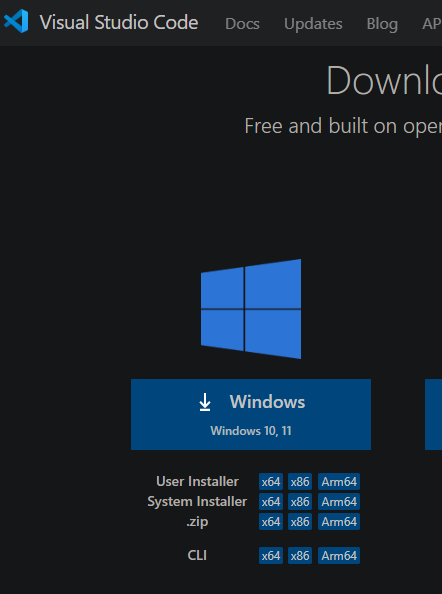
\includegraphics[width=3in]{images/windowsVSCodeSetup/image6.png}
    
    \item Run the installer and accept all of the default settings.
    \item Click on Install and wait for Visual Studio Code to finish installing, then close the installer.
\end{itemize}
\subsubsection{Step 2: Installing MinGW}
This section is based on this guide from Microsoft: \textcolor{cyan}{\href{https://code.visualstudio.com/docs/cpp/config-mingw}{https://code.visualstudio.com/docs/cpp/config-mingw}}

MinGW is a Windows C/C++ compiler tool set that will allow us to compile our C/C++ code into a .exe file.

\begin{itemize}
    \item First Install MinGW from \textcolor{cyan}{
    \href{https://github.com/msys2/msys2-installer/releases/download/2023-05-26/msys2-x86_64-20230526.exe}{this link}}
    \item Open the installer and choose the Defaults for all settings.
    \item At the end of the installation run msys2 and then run the following command:
    
    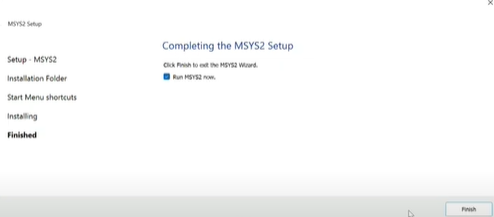
\includegraphics[width=6in]{images/windowsVSCodeSetup/image8.png}
    
    (Shift + Insert is the paste shortcut in MSYS2’s terminal)
    \begin{minted}{bash}
        pacman -S --needed base-devel mingw-w64-x86_64-toolchain
    \end{minted}
    
    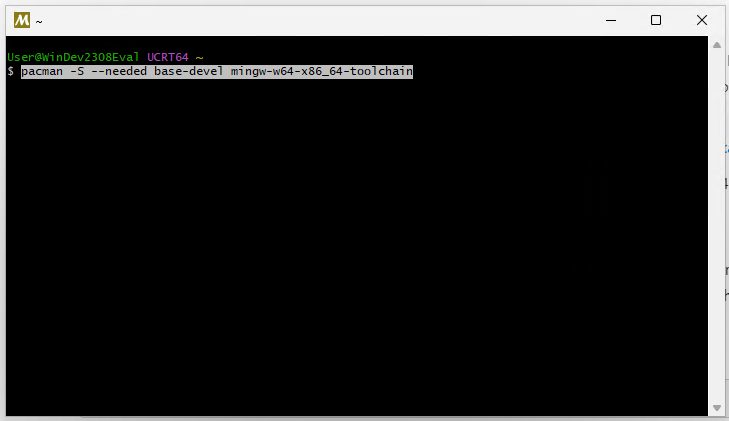
\includegraphics[width=6in]{images/windowsVSCodeSetup/image7.png}
    
    \item Press enter when prompted to install all of the default packages, then press Y to confirm the install. This will take 1 to 5 minutes to finish. Once the install completes you can close msys2.
    \item Now we need to add msys2 to window’s PATH variable. Press the Windows key and begin typing  “Edit environment variables for your account” until you see this option.

    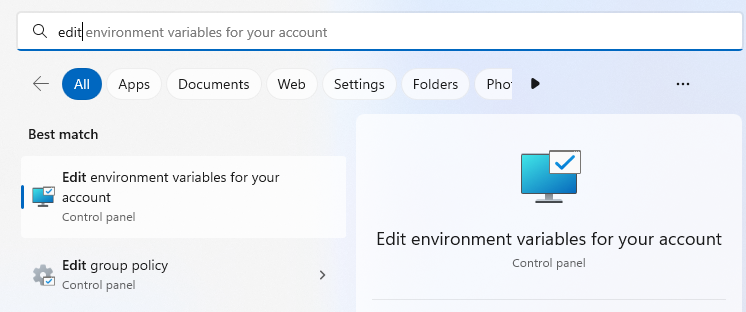
\includegraphics[width=5in]{images/windowsVSCodeSetup/image10.png}

    Now Select the “PATH” variable and click edit, in the window that opens click “New” and enter the following path for the default installation location of Msys2.
    
    \begin{minted}{bash}
        C:\msys64\mingw64\bin
    \end{minted}

    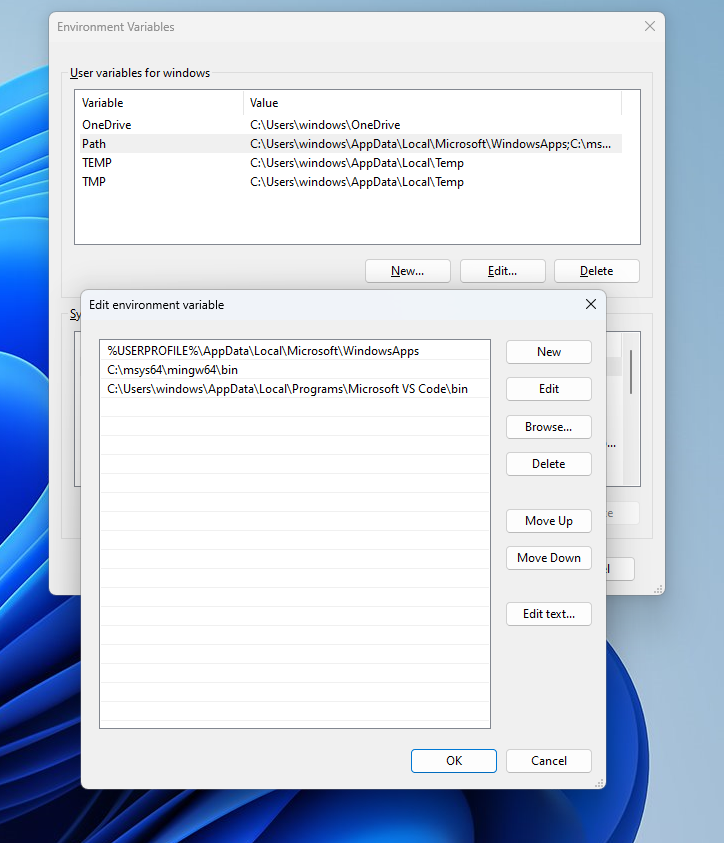
\includegraphics[width=4in]{images/windowsVSCodeSetup/image9.png}
     
\end{itemize}

\subsubsection{Step 3: Adding VS code extensions}

\begin{itemize}
    \item After you Reboot open VScode and select the extensions tab. (5th from the top), and search for ``C++". We need to install the ``C/C++" and “C/C++ Extension Pack” both from Microsoft.

    
\includegraphics[width=3in]{images/windowsVSCodeSetup/image12.png}

    \item Select the extension then click on install, these will provide Syntax Highlighting and other useful tools when working in C++

    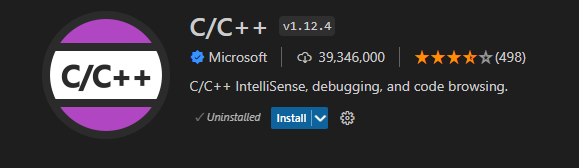
\includegraphics[width=5in]{images/windowsVSCodeSetup/image11.png}

    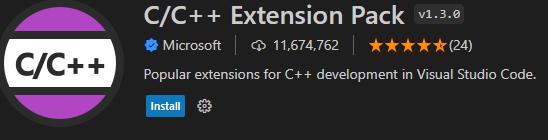
\includegraphics[width=5in]{images/windowsVSCodeSetup/image14.png}
\end{itemize}

\subsection{Mac Installation}

\subsubsection{Step 1: Installing VS Code}

\begin{itemize}
    \item Go to \textcolor{cyan}{\href{VS code download page}{https://code.visualstudio.com/Download}} , and download for Mac. 

    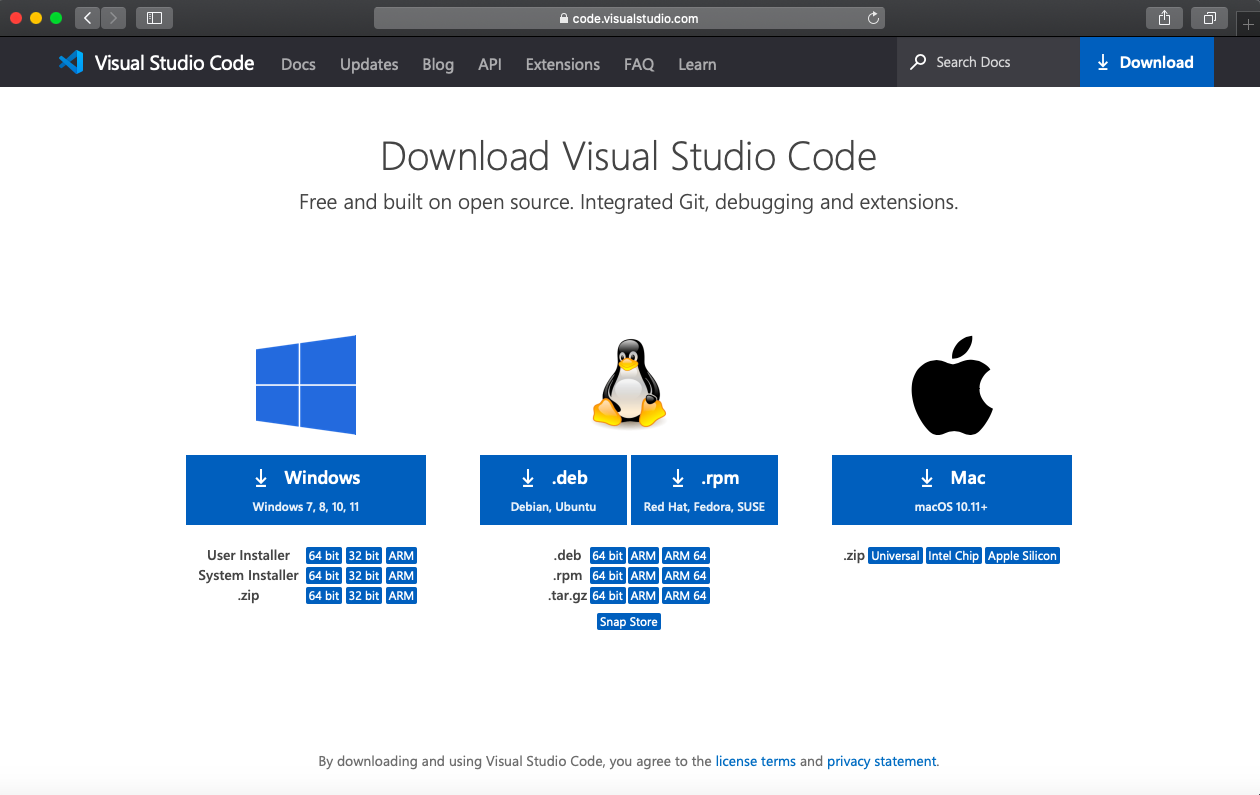
\includegraphics[width=6in]{images/macVSCodeSetup/image3.png}

    \item After the download has finished, unzip the folder by double-clicking on it.

    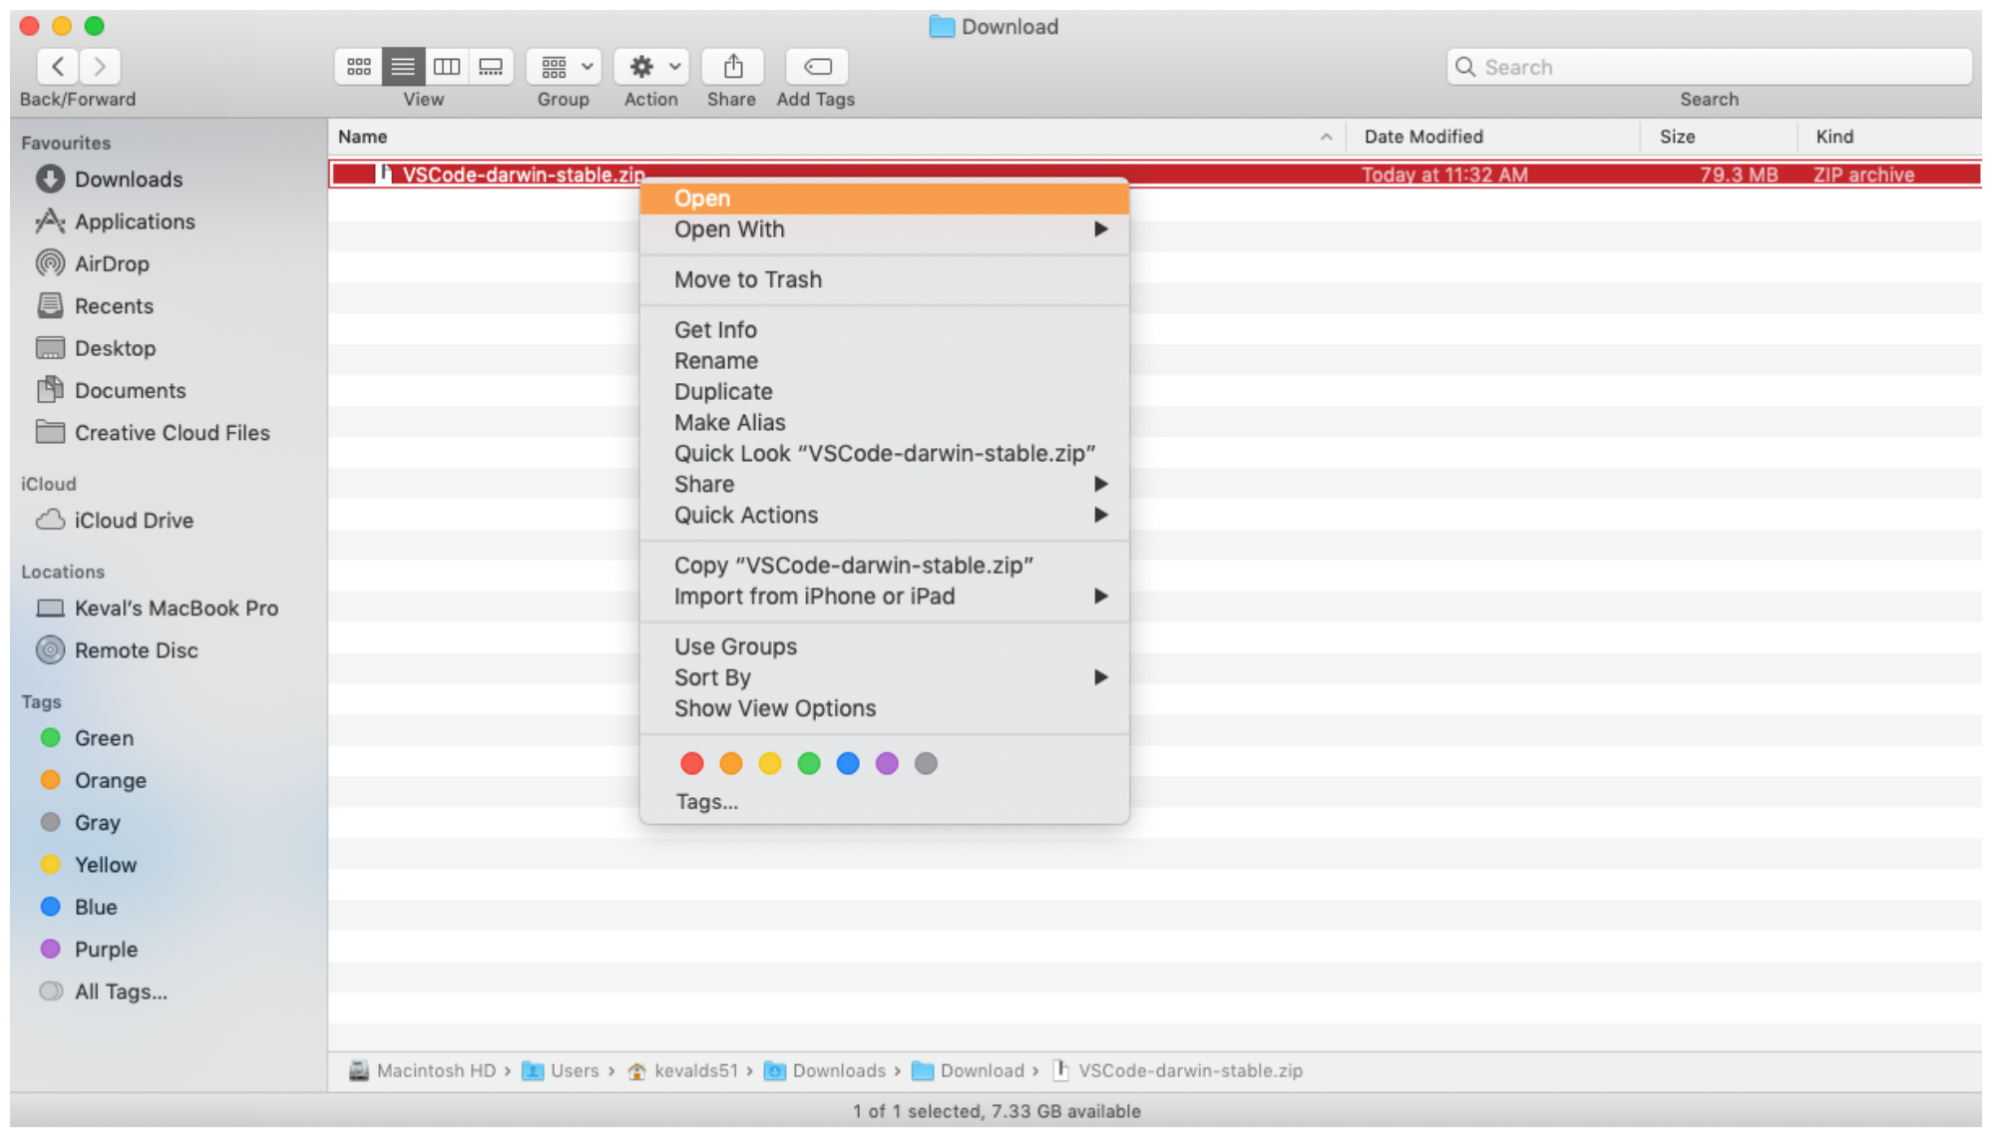
\includegraphics[width=6in]{images/macVSCodeSetup/image5.png}

    \item Now you can see the “Visual Studio Code” application. Drag and drop this icon to the “Applications” folder of your computer. 

    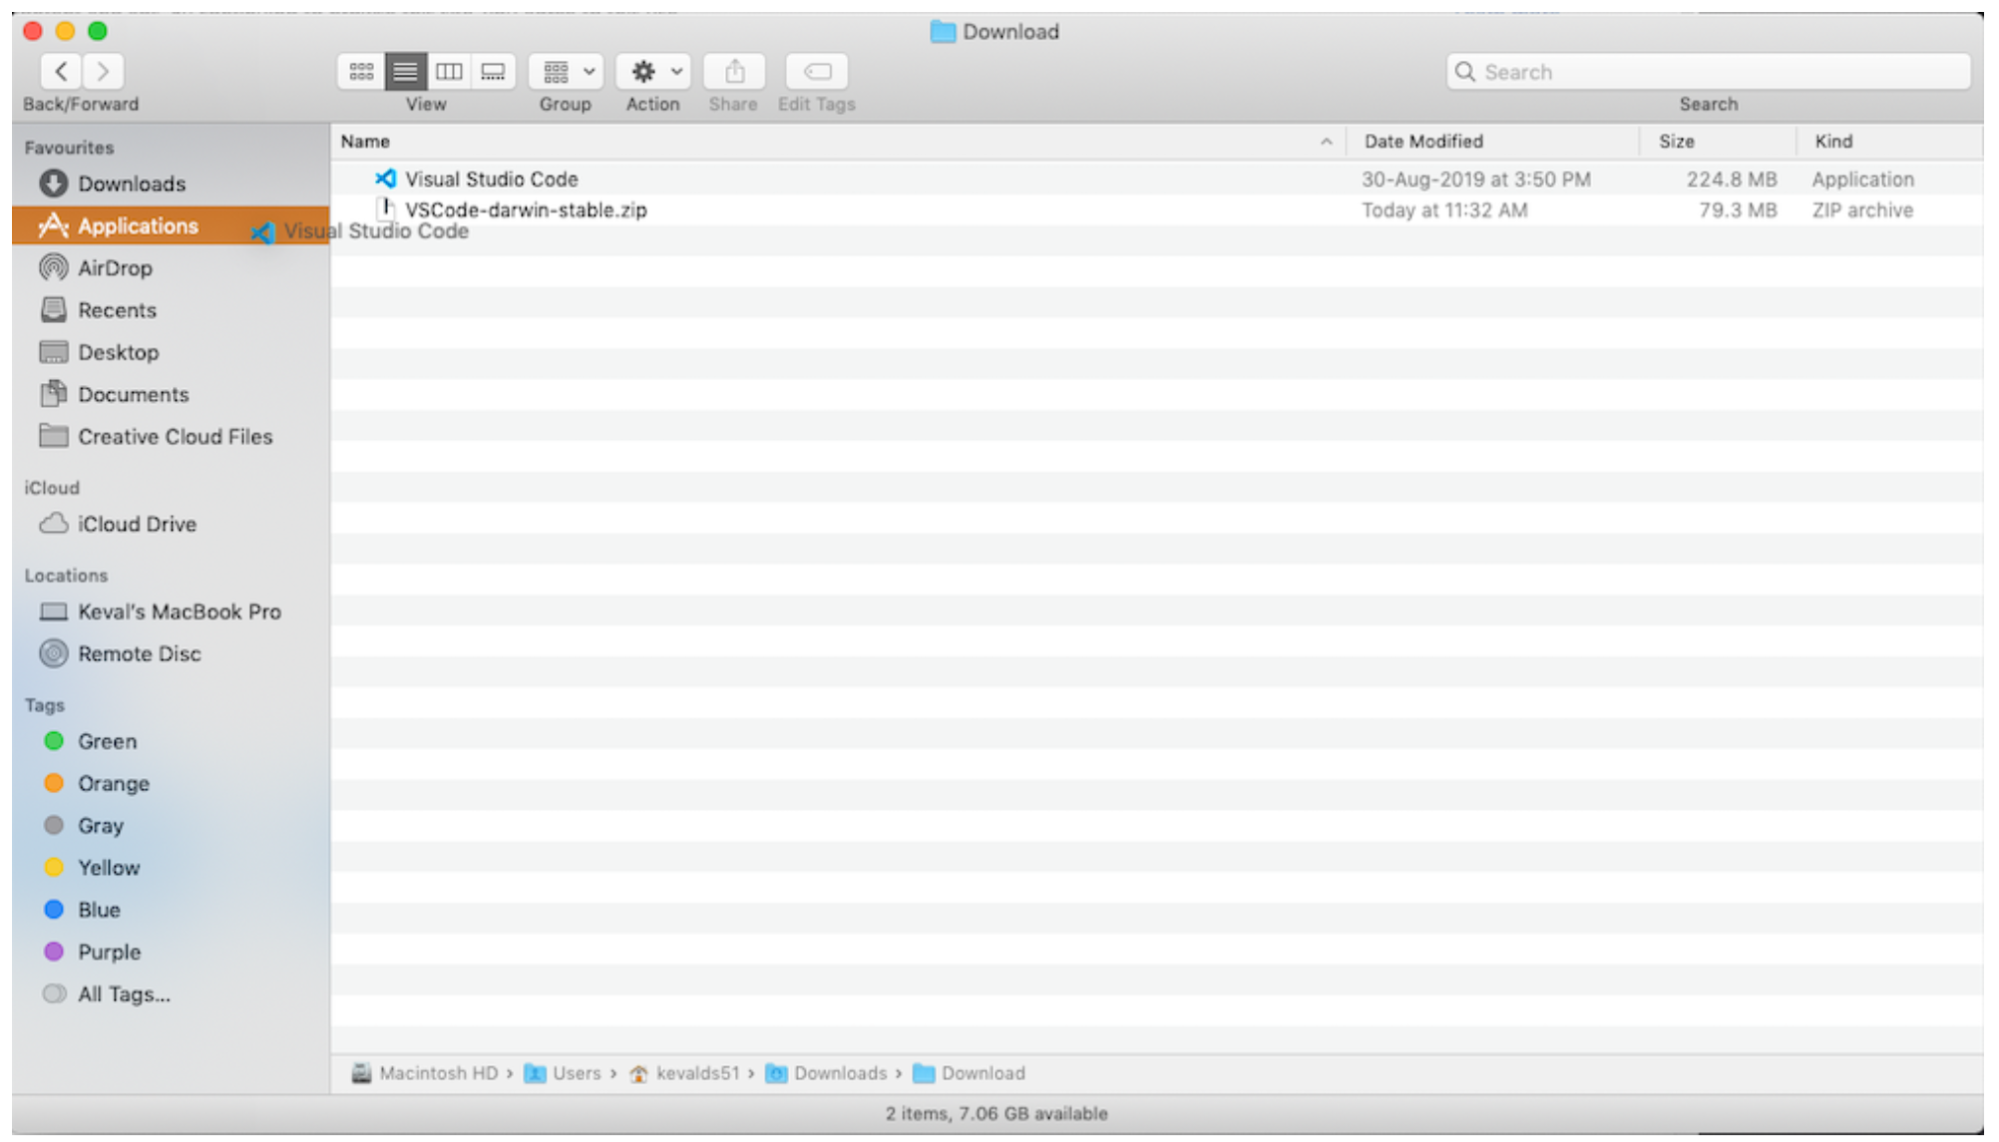
\includegraphics[width=6in]{images/macVSCodeSetup/image4.png}

    \item Double click on the ”Visual Studio Code” icon to launch the application. (You might need to right click and select “open” if you cannot launch the program). Next, select the ”New Terminal” option to open the terminal window.

    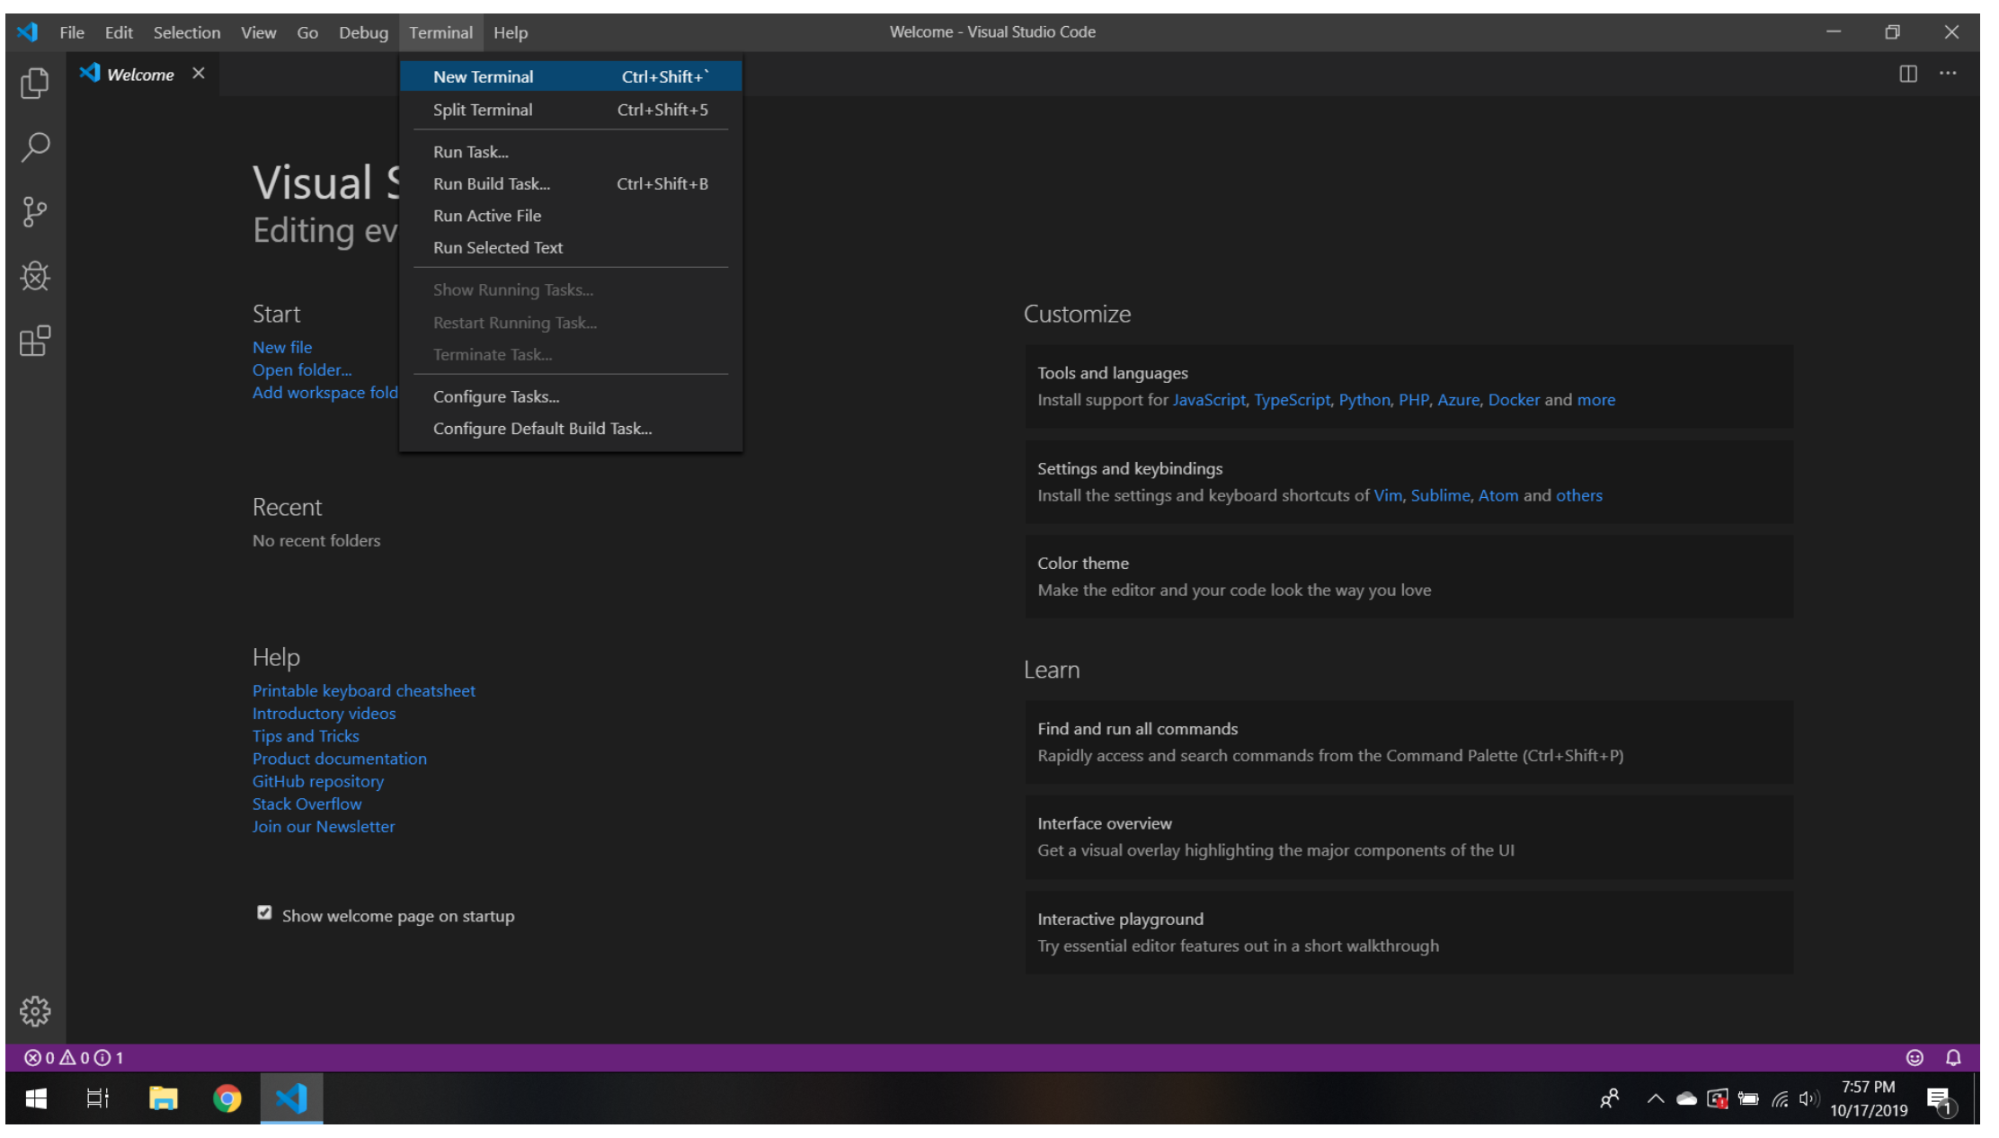
\includegraphics[width=6in]{images/macVSCodeSetup/image7.png}

    \item Install C/C++ extension. In the toolbar on the left hand side of the screen click on the bottom icon for Extensions. Search for C/C++ and click install.

    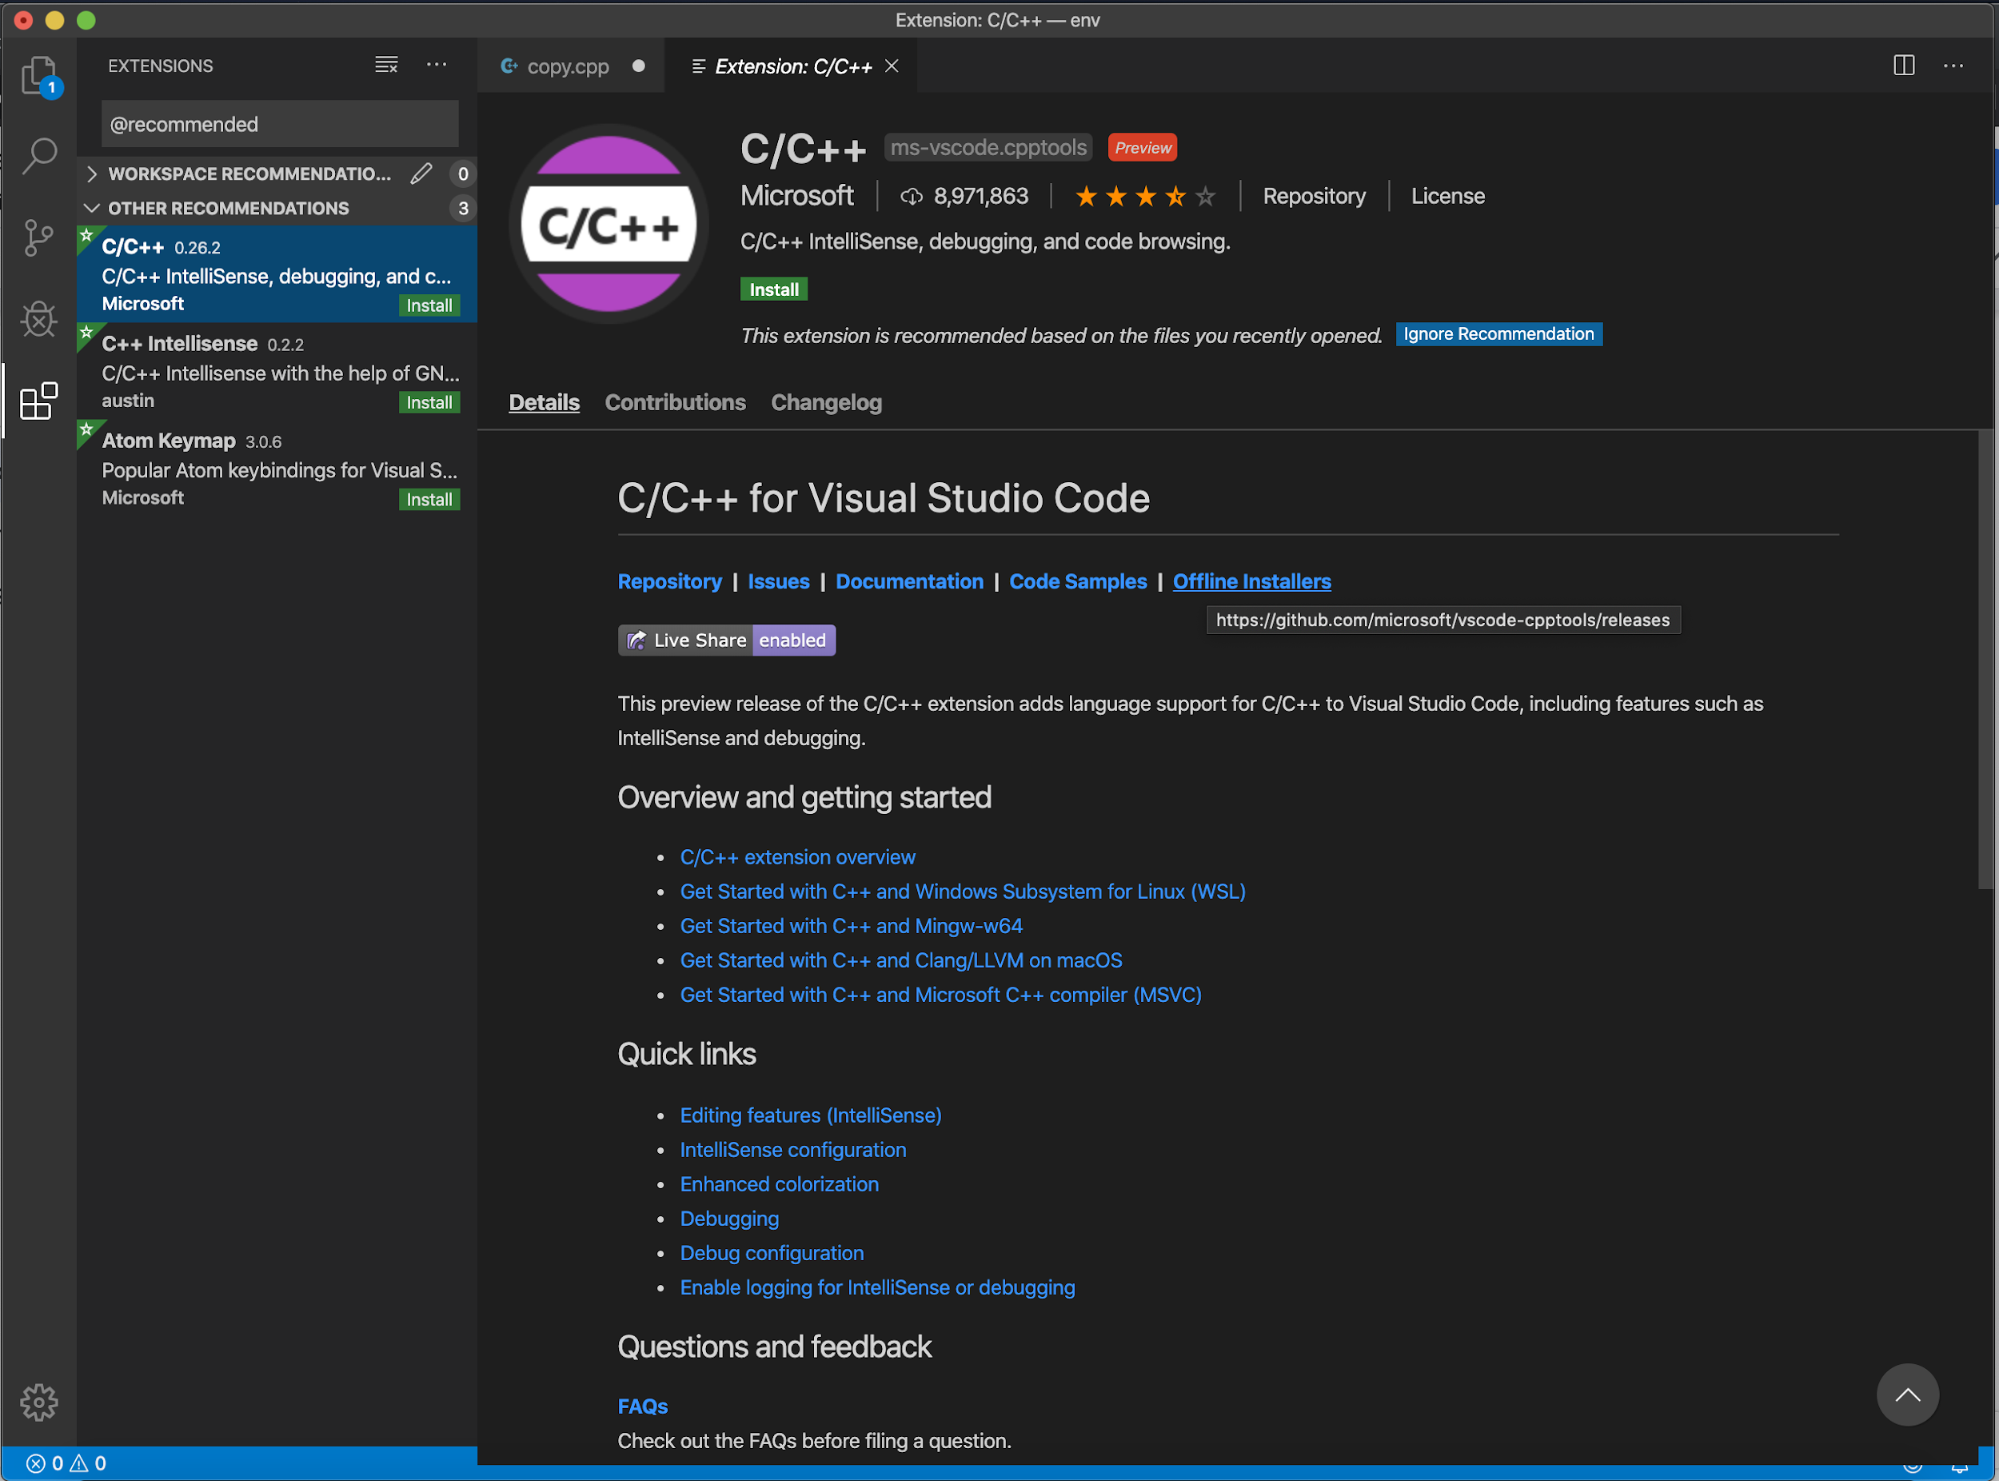
\includegraphics[width=6in]{images/macVSCodeSetup/image6.png}

\end{itemize}

\subsubsection{Step 2: Install g++}

\begin{itemize}
    \item Open a Terminal window.(One way is to press Command+Space, type Terminal in the search field, and press the Return key.)
    \item In the Terminal window type \mintinline{c++}{g++} and press the Return key. We will see an alert box like this:

    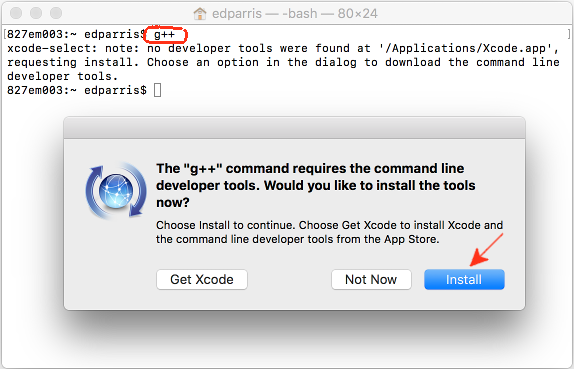
\includegraphics[width=4in]{images/macVSCodeSetup/image9.png}

    \item Choose Install to get only the command line tools unless you want to learn Xcode.
    
    Xcode can be installed later from the App Store.
    
    After installation, type g++ in the Terminal, press the Return key, and verify the terminal prints the message, "no input files".
    \begin{minted}{bash}
    $ g++
    clang: error: no input files
    \end{minted}

    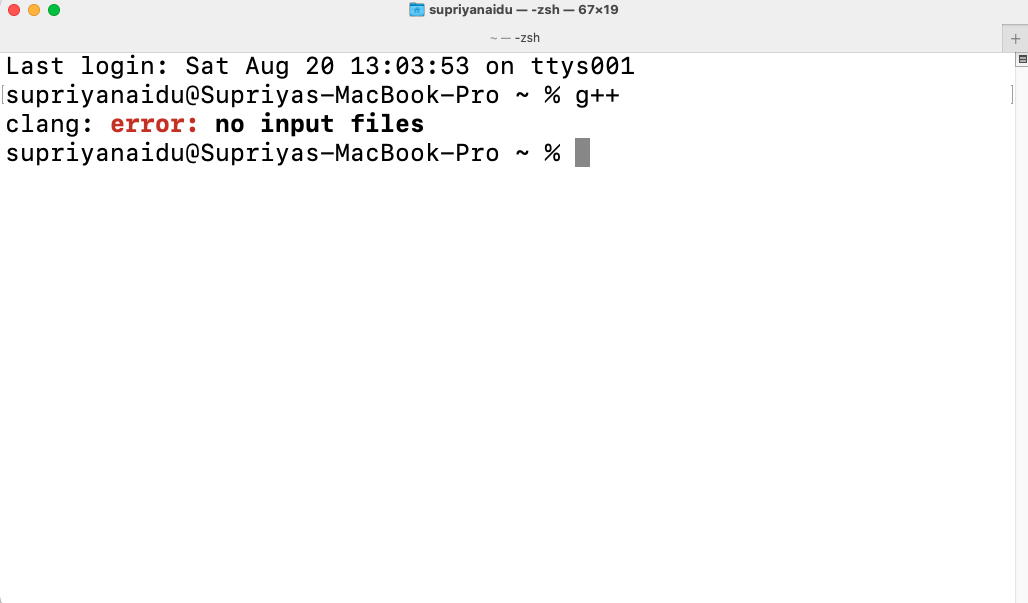
\includegraphics[width=4in]{images/macVSCodeSetup/image8.png}
\end{itemize}


\section{Debugger Installation}

A debugger is an incredibly powerful tool you can use to help find issues with your code and fix them. It allows you to do step-by-step examination of your code, inspecting variable values at different points, and understanding how your code actually runs when it is executed.

\subsection{Windows Installation}

Windows users will use a debugger called gdb to debug their C++ code. This program has been installed with your compiler in homework0. The steps below will demonstrate the process of setting up the debugger in VSCode on Windows.

\subsubsection{Step 1: Open Code Directory with VS Code}

Begin by opening VS Code. Open the folder containing your code. For demonstration purposes, we will be using the ``csci1300" folder located in Desktop. Once you have navigated to the target folder and selected it, click ``Select Folder" on the lower right corner of the folder selection dialog. You should see something resembling the image below. 

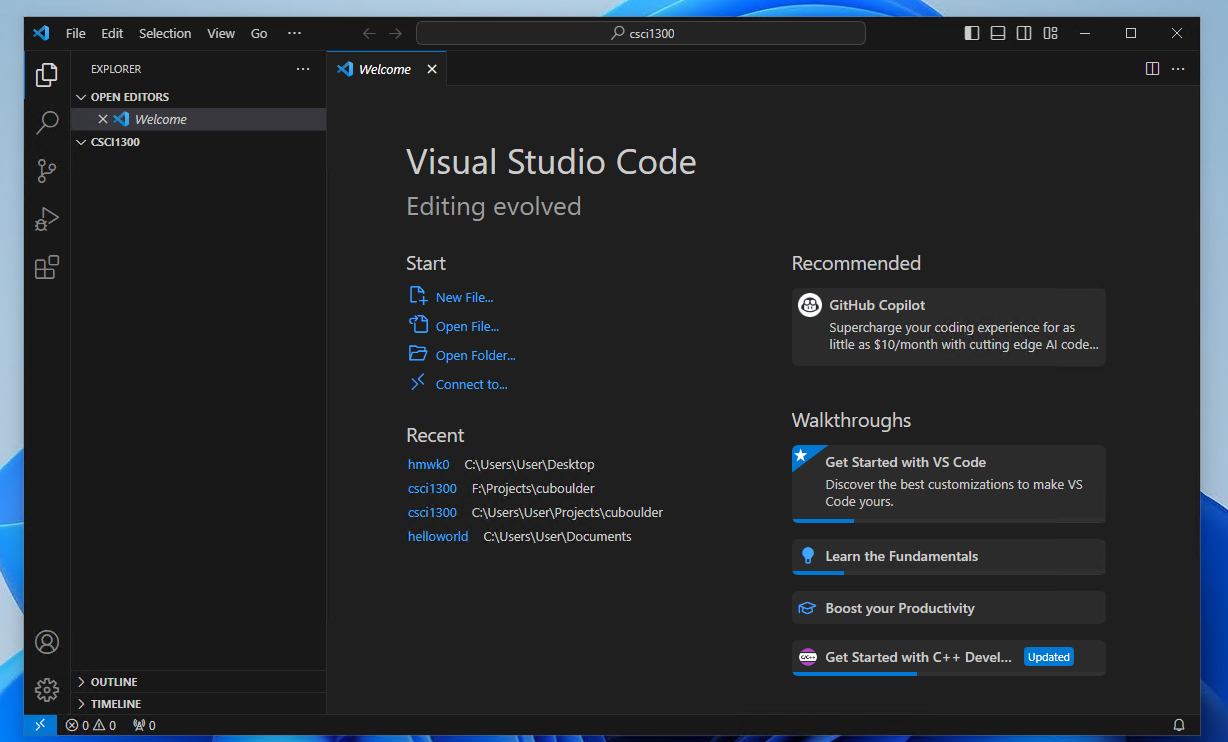
\includegraphics[width=\textwidth]{images/windowsDebuggerSetup/debugger_windows_1.png}

\subsubsection{Step 2: Open A File to Debug}

If you already have a cpp file in this folder, double click that file in the left pane. In this demonstration, we will be creating a new cpp file named ``hello\_world.cpp". 

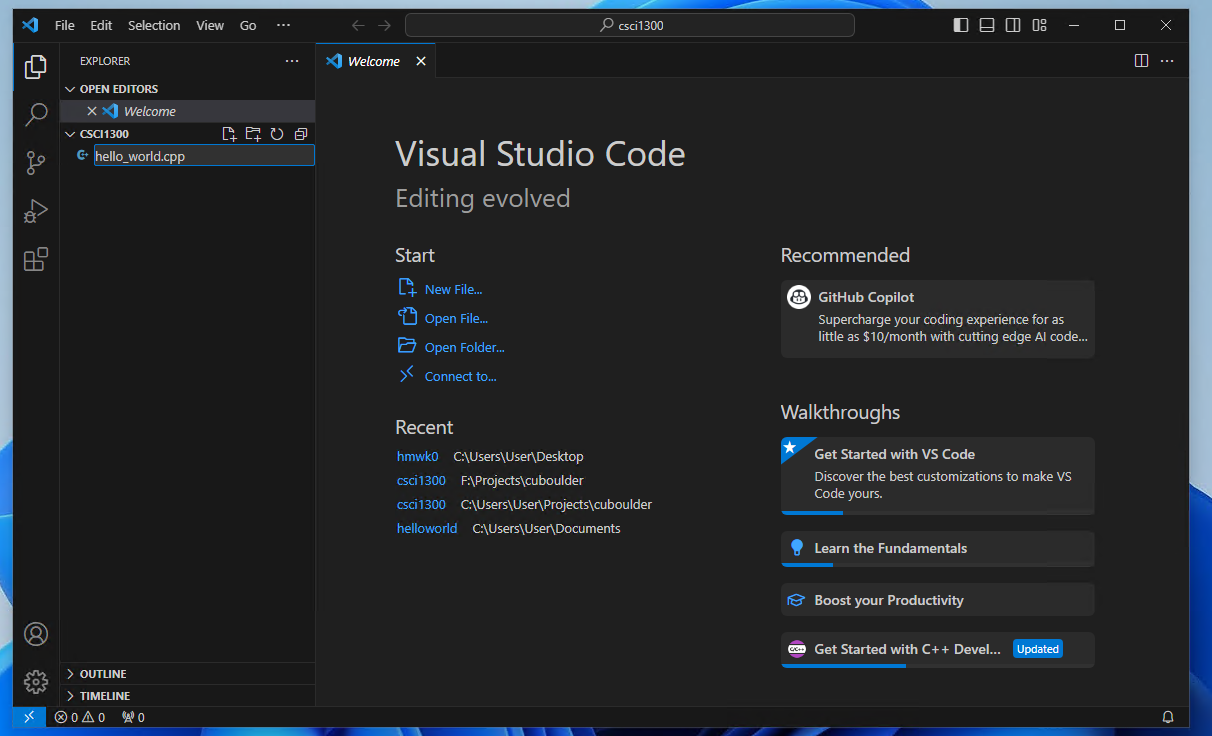
\includegraphics[width=\textwidth]{images/windowsDebuggerSetup/debugger_windows_2.png}

The sample code we will be using is as follows. This code declares a string variable named ``message" and prints it to the terminal.

\begin{minted}{c++}
#include <iostream>
using namespace std;

int main()
{
    string message = "Let's Debug!";
    cout << message << endl;
    return 0;
}
\end{minted}

Copy the sample code into ``hello\_world.cpp" and save the file. 

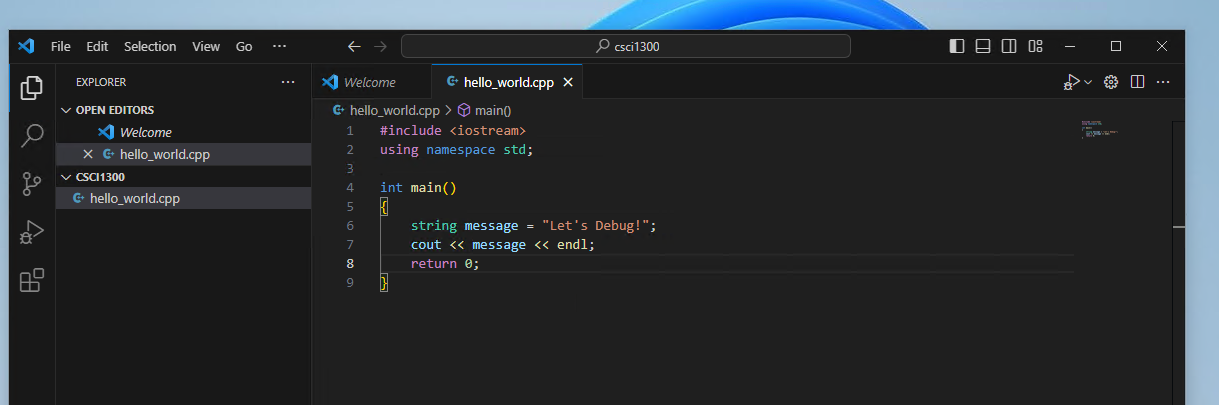
\includegraphics[width=\textwidth]{images/windowsDebuggerSetup/debugger_windows_3.png}

\subsubsection{Step 3: Click ``Run and Debug"}

Go to the debugging pane by clicking on the icon in the red square. Then click ``Run and Debug". 

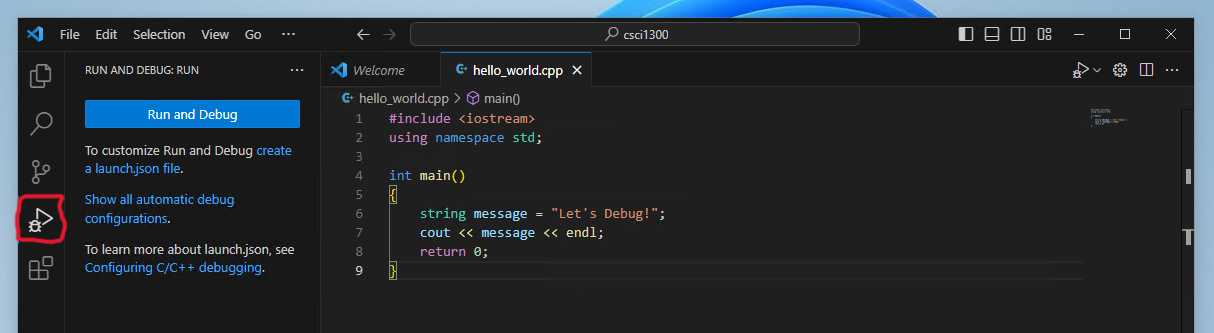
\includegraphics[width=\textwidth]{images/windowsDebuggerSetup/debugger_windows_4.png}

\subsubsection{Step 4: Select Debugging Option}

After clicking ``Run and Debug", a dialog will appear as shown below.
Select ``C++ (GDB/LLDB)" 

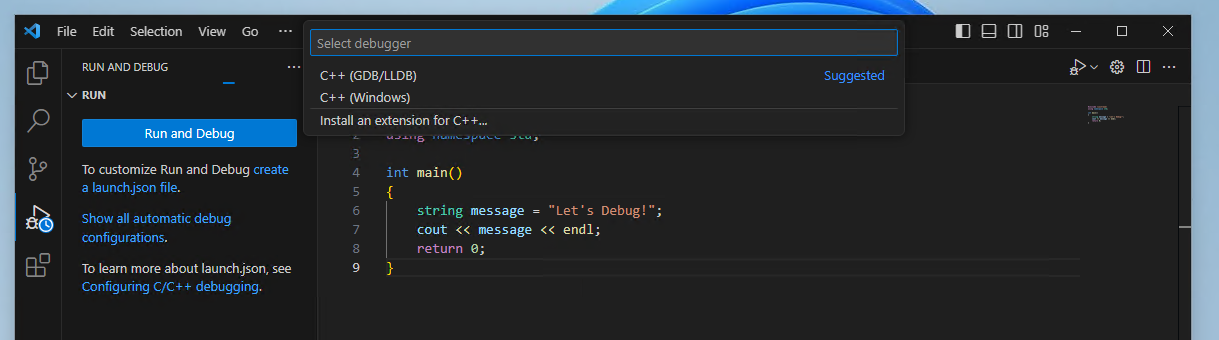
\includegraphics[width=\textwidth]{images/windowsDebuggerSetup/debugger_windows_5.png}

Another dialog will show up as shown below.
Select the option that contains \mintinline{bash}{C:\msys64\mingw64\bin\g++.exe}

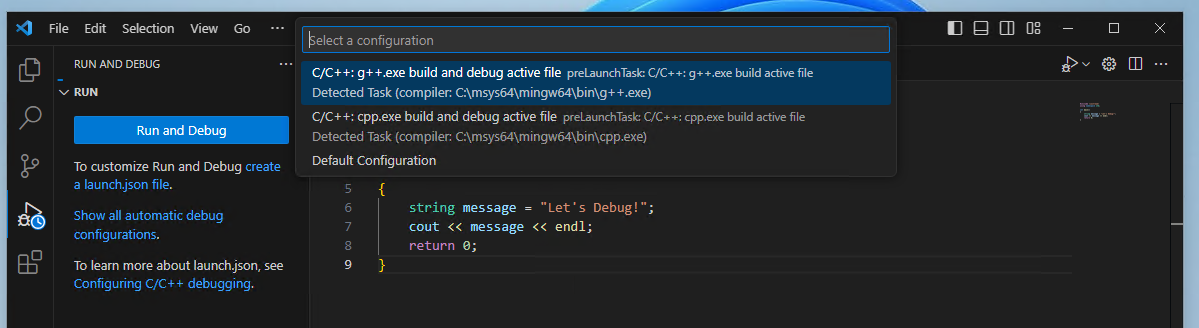
\includegraphics[width=\textwidth]{images/windowsDebuggerSetup/debugger_windows_6.png}

The result will be as shown below. For the dialog at the bottom right corner of the screen click ``Not now". 

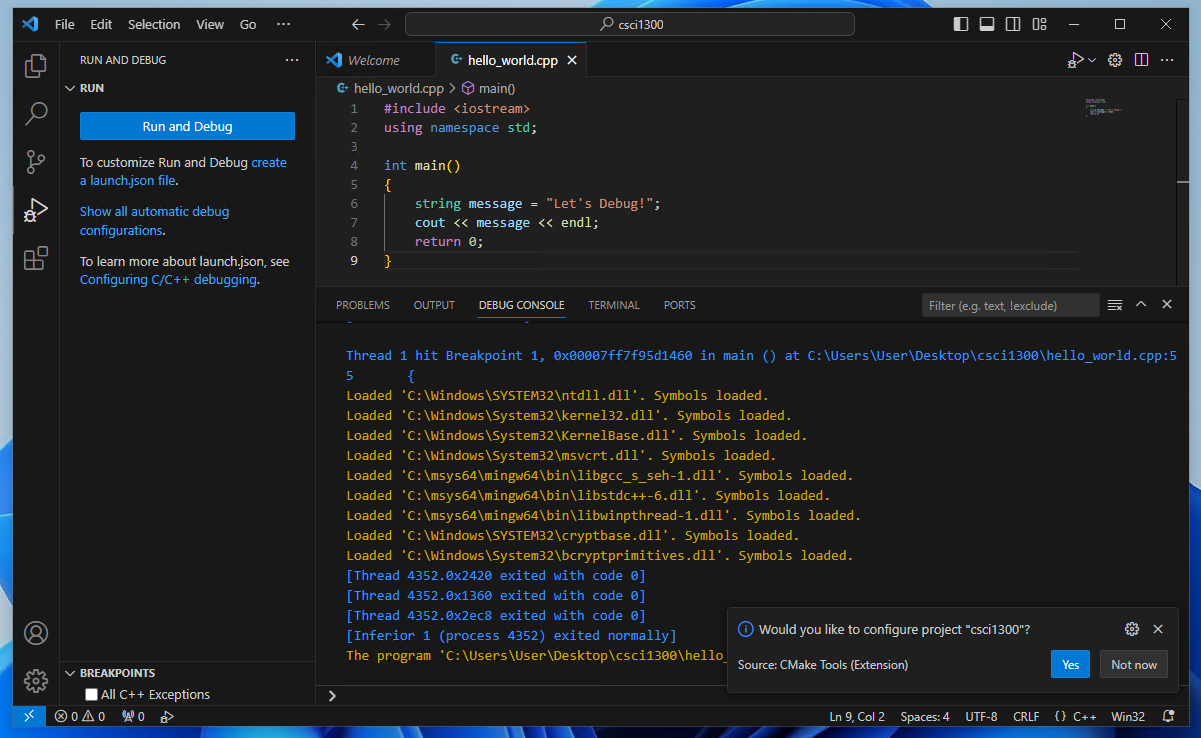
\includegraphics[width=\textwidth]{images/windowsDebuggerSetup/debugger_windows_7.png}

Click ``TERMINAL" in the center of the screen. You will see the message in the terminal ``Let's Debug!". At this point you have successfully setup and ran your debugger in VSCode. To make the debugger to the same compilation flags that we use, we will have to edit a configuration file called ``tasks.json". 

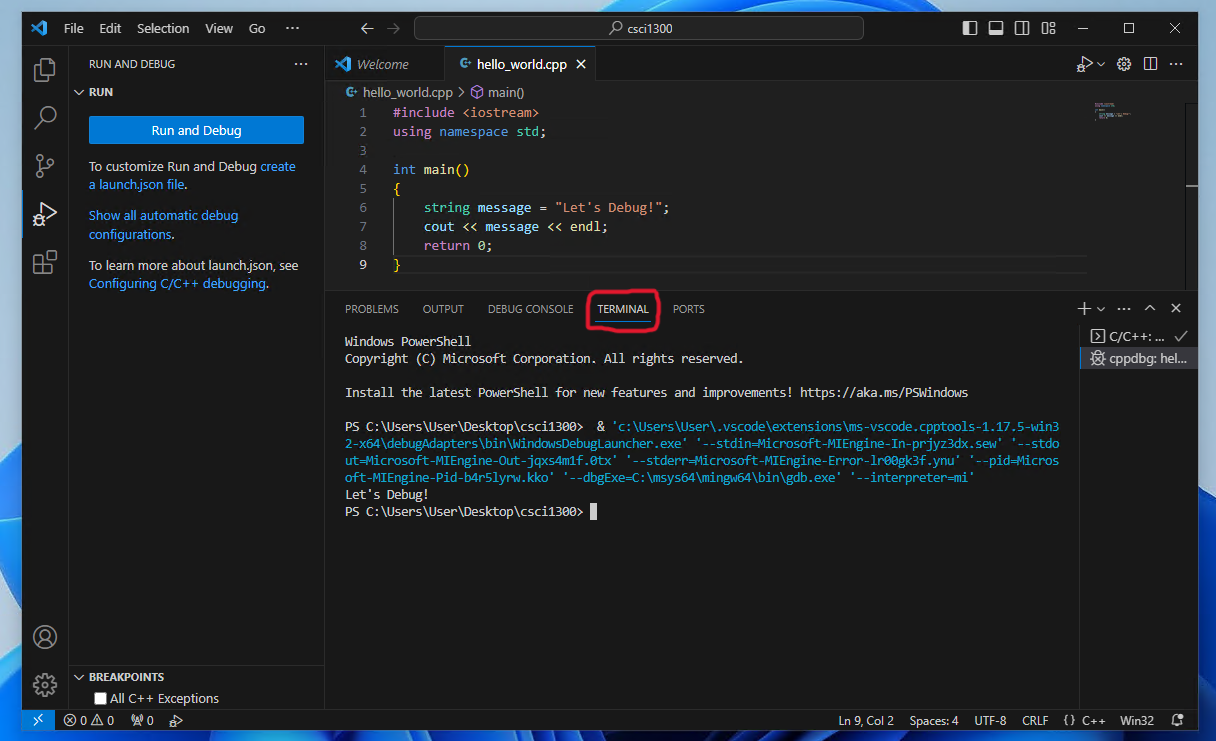
\includegraphics[width=\textwidth]{images/windowsDebuggerSetup/debugger_windows_8.png}

Navigate back to the file explorer pane by clicking the first icon on the left pane. There will be a folder with the name ``.vscode" created for you. 

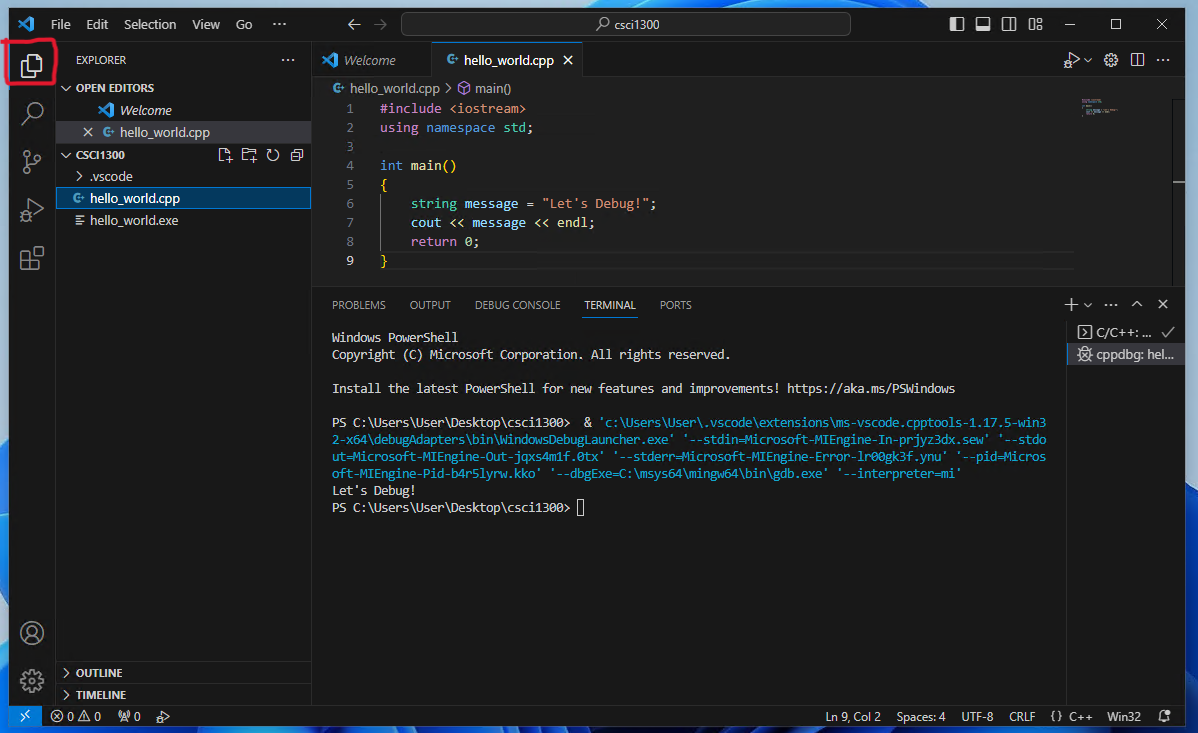
\includegraphics[width=\textwidth]{images/windowsDebuggerSetup/debugger_windows_9.png}

Click the folder to view the files inside. You will find ``tasks.json" inside. 

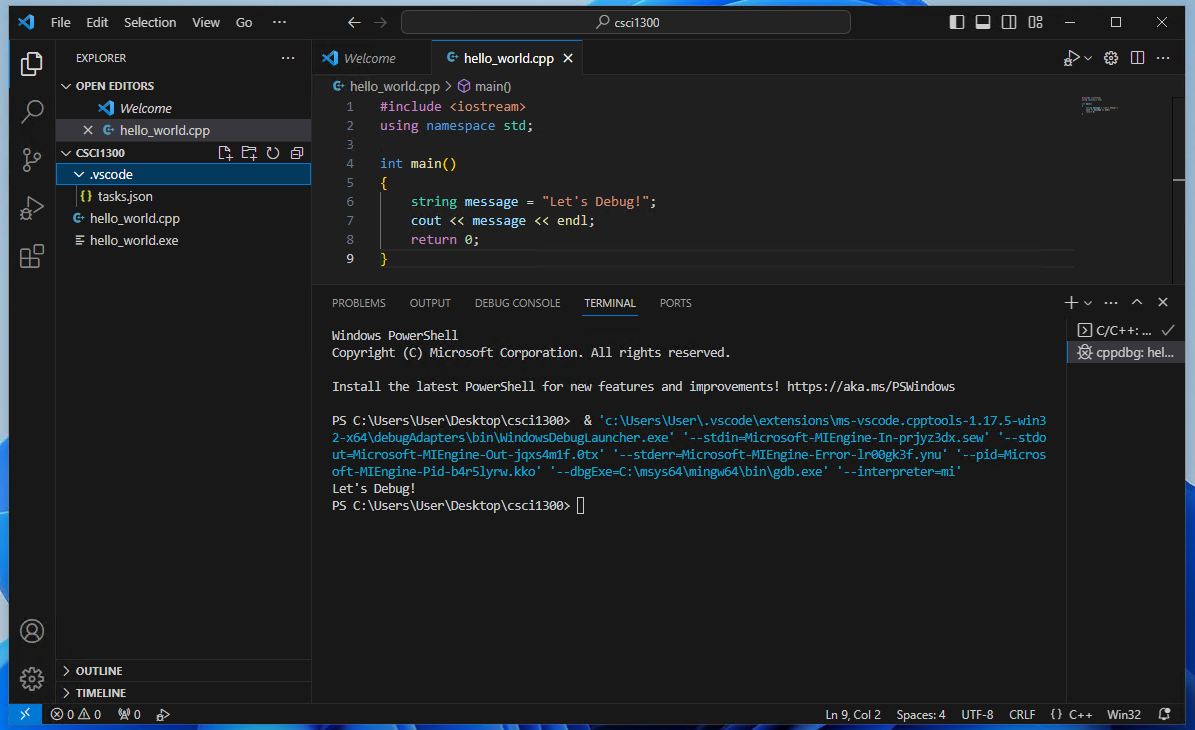
\includegraphics[width=\textwidth]{images/windowsDebuggerSetup/debugger_windows_10.png}

Open ``tasks.json". This is the configuration of your debugging task which include compilation commands. 

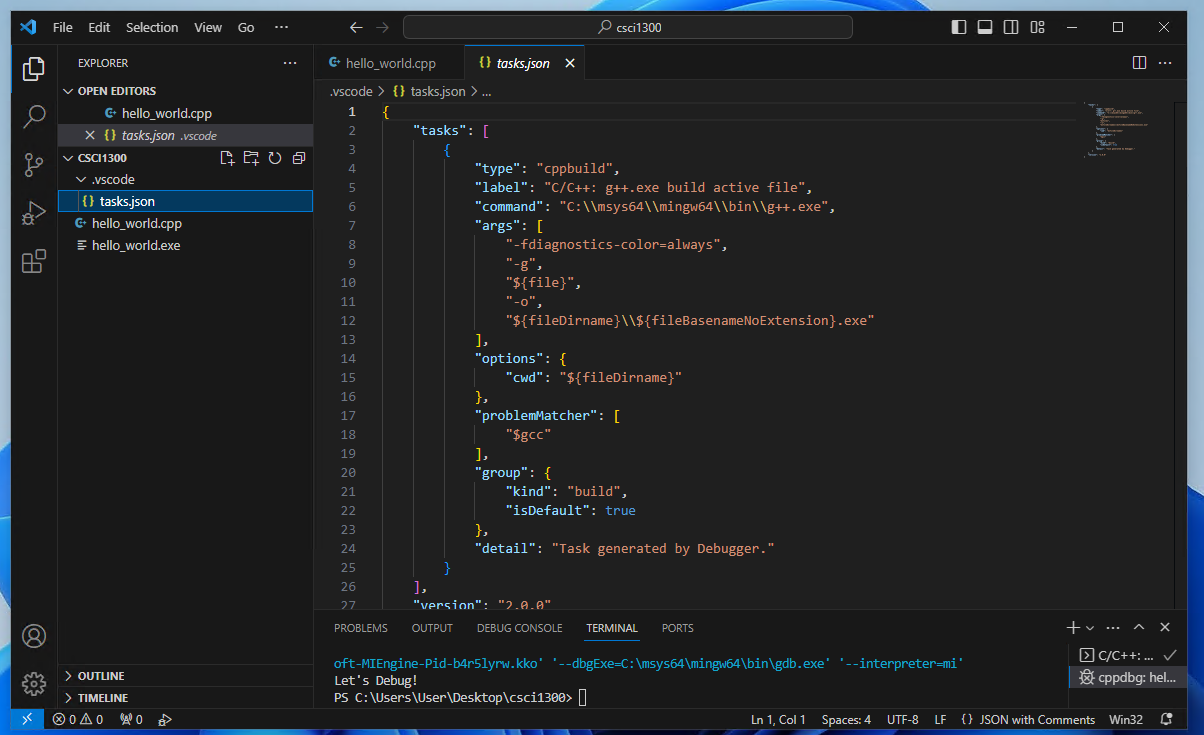
\includegraphics[width=\textwidth]{images/windowsDebuggerSetup/debugger_windows_11.png}

Add the values ``-Wall", ``-Werror" and ``-Wpedantic" in the ``args" section as shown below. Save the file after you have completed editing. 

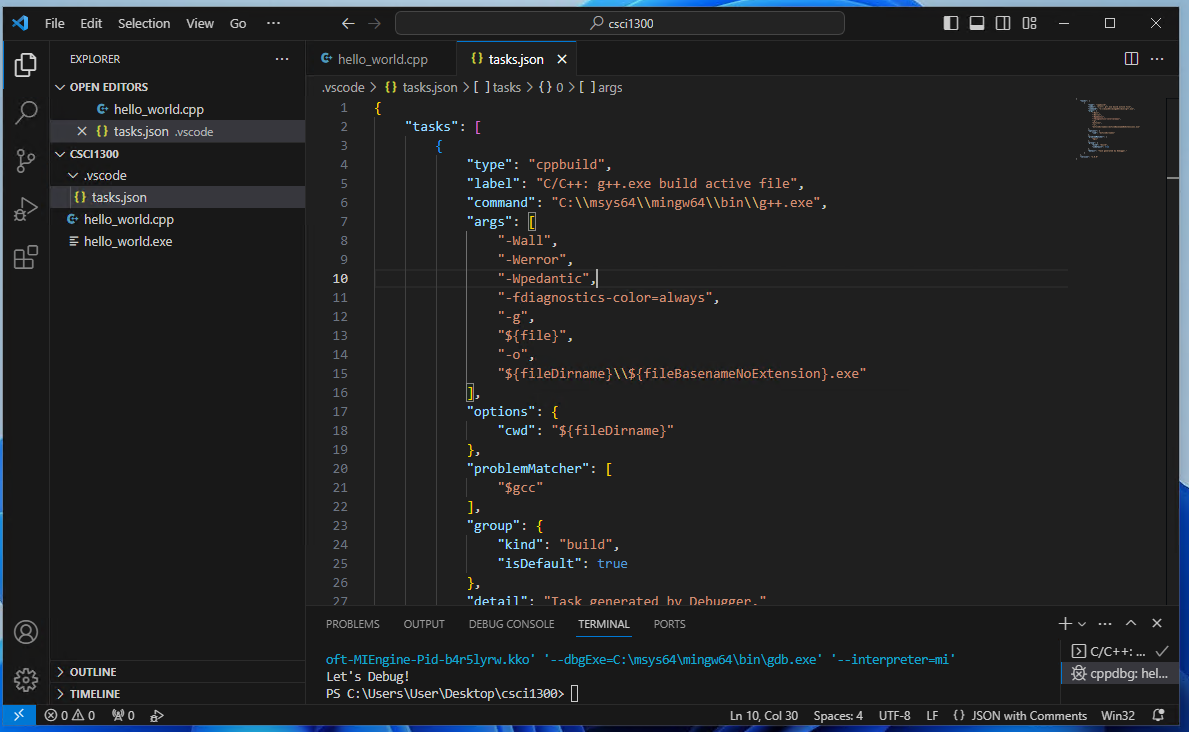
\includegraphics[width=\textwidth]{images/windowsDebuggerSetup/debugger_windows_12.png}

\subsubsection{Step 5: Adding breakpoints}

Breakpoints are line or specific code that we want to inspect. Once a breakpoint is reached during runtime, the program will pause for you to inspect the value of each variable. Once you are done inspecting that particular point, you may continue the program by pressing continue.

Navigate back to your cpp file by clicking the tab of you file at the center top of the screen. To add a breakpoint, hover your mouse over the line number of your code that you would like to inspect. The image below is selecting line 7. After clicking, the red dot will not disappear when you move your mouse away.

\begin{table}[H]
    \centering
    \begin{tabular}{c|c}
        Selecting line of code & Breakpoint added to line of code \\
        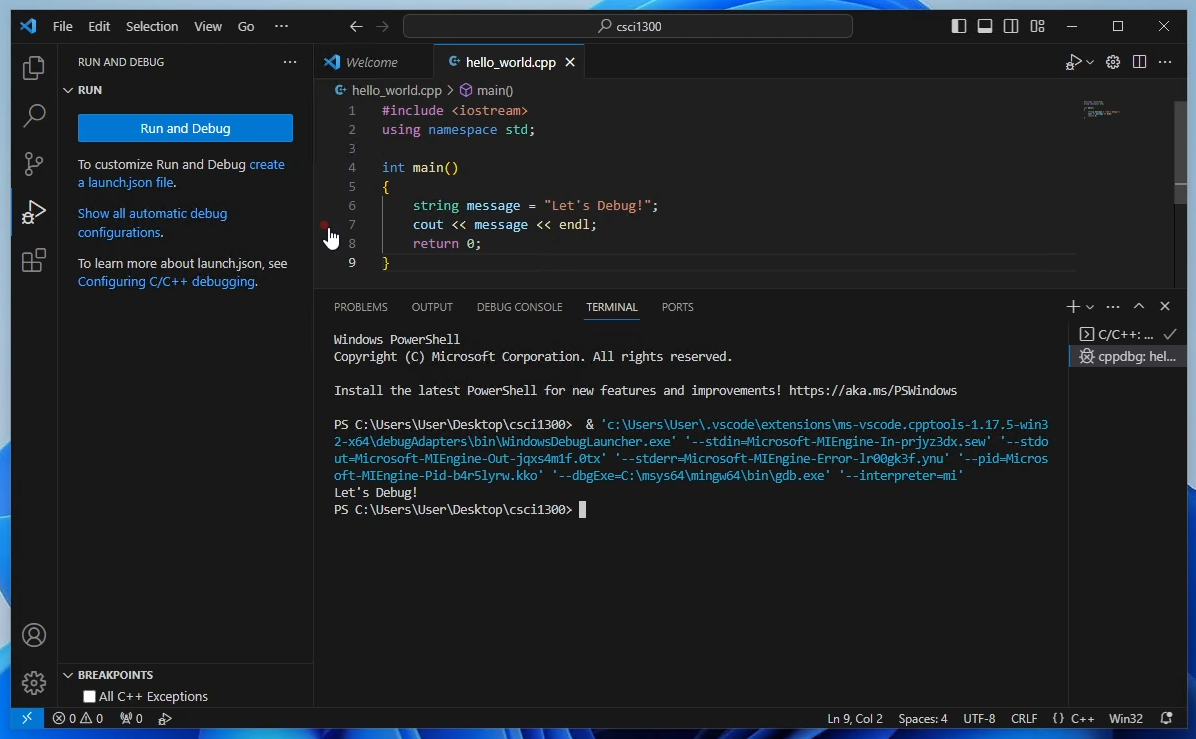
\includegraphics[width=0.5\textwidth]{images/windowsDebuggerSetup/debugger_windows_13.png} & 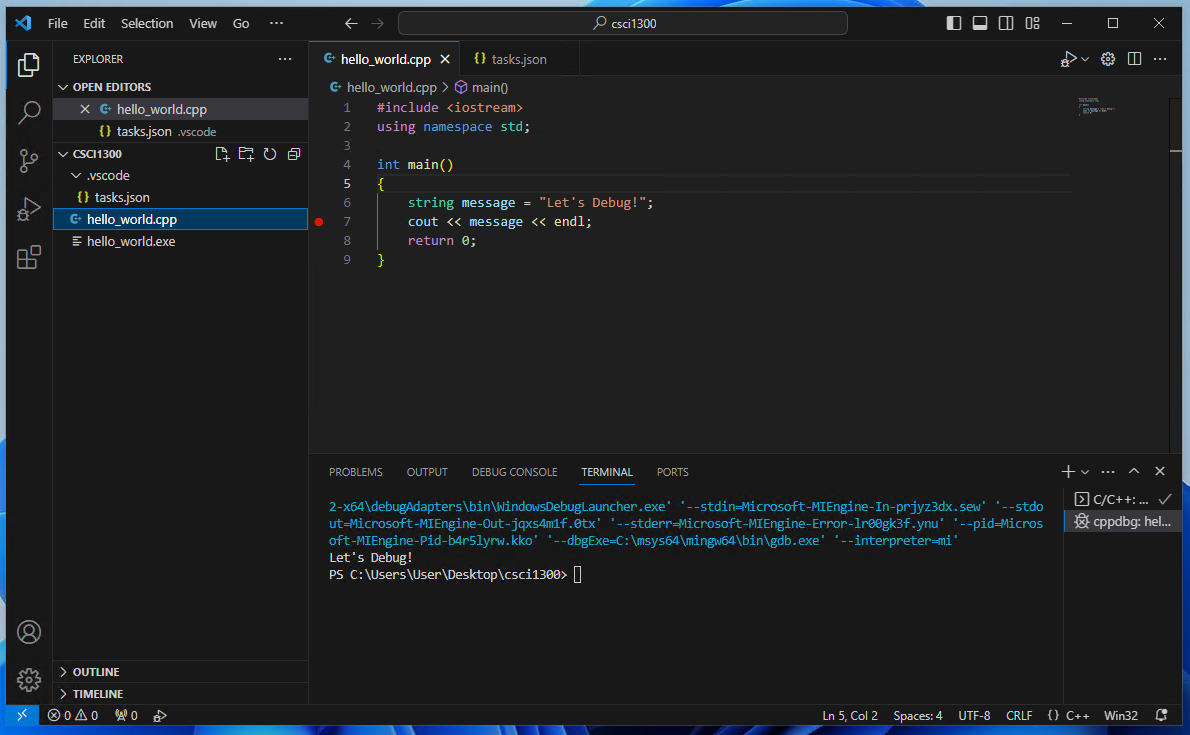
\includegraphics[width=0.5\textwidth]{images/windowsDebuggerSetup/debugger_windows_14.png}
    \end{tabular}
\end{table}

Now we can run the debugger by navigating to the debugging pane and clicking "Run and Debug" as in step 3 and 4. 

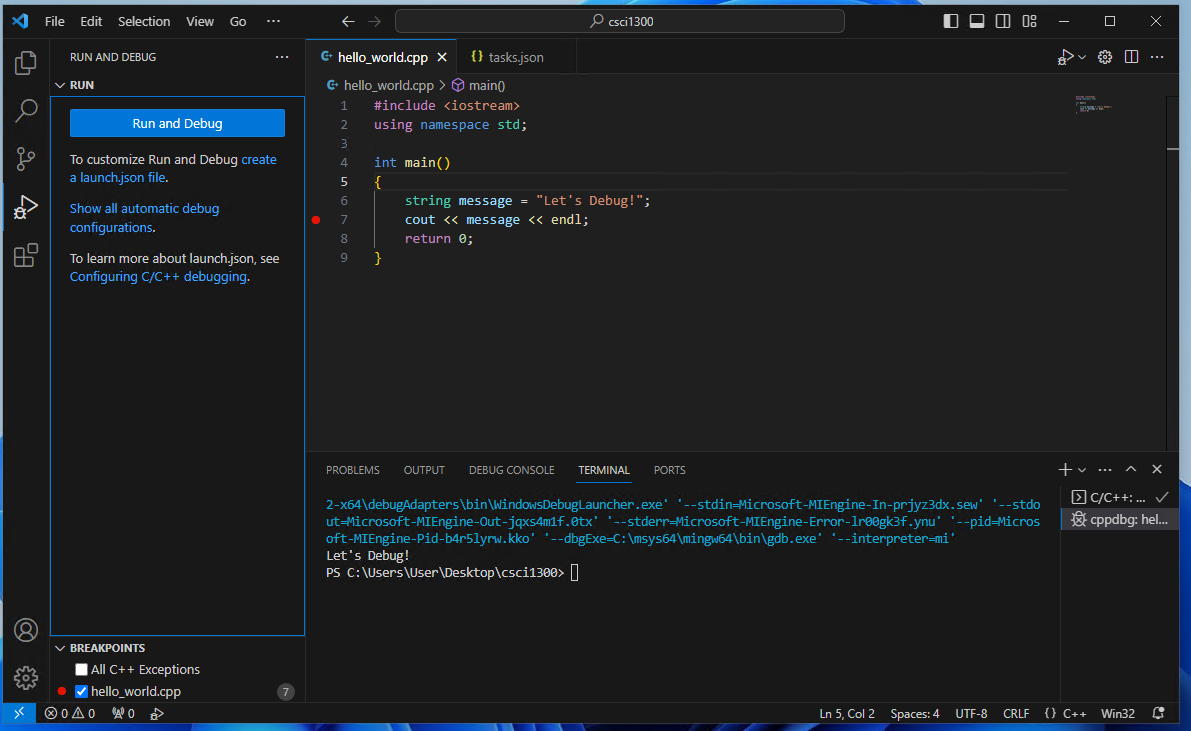
\includegraphics[width=\textwidth]{images/windowsDebuggerSetup/debugger_windows_15.png}

Notice that our program pauses at the line the breakpoint was added. There is also a list of variables on the left pane. For this instance, the variable ``message" is being shown with the value ``Let's Debug!". This is very useful when we have many variables in our program. 

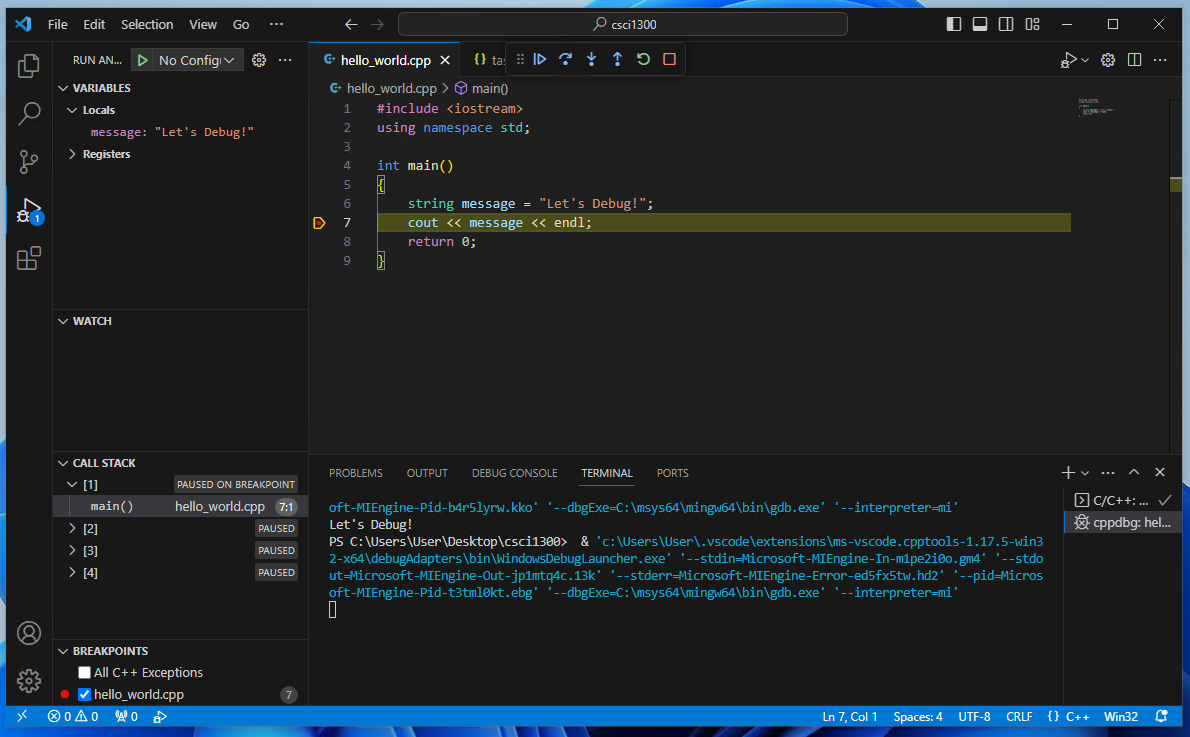
\includegraphics[width=\textwidth]{images/windowsDebuggerSetup/debugger_windows_16.png}

The menu to control the execution of your program looks like this:

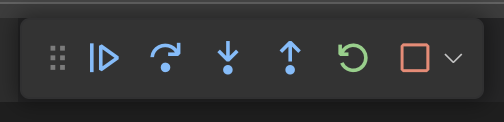
\includegraphics[width=0.3\textwidth]{images/windowsDebuggerSetup/debugger_windows_17.png}

The buttons, left to right, are as follows:

\begin{itemize}
    \item Continue: go until the next breakpoint is encountered
    \item Step Over: go to the next line, skipping the details of functions
    \item Step Into: go to the next line, if necessary jumping into a function that is called
    \item Step Out: jump to the end of the function your are in, returning to wherever that function was called from
    \item Restart: start the program over from the beginning
    \item Stop: quit debugging
\end{itemize}

Most of the time you can do most of your debugging with just the Continue and the Step Over buttons as long as you have put breakpoints at all the points of your code you care about.

\subsection{Mac Installation}

MacOS users will use a debugger called lldb to debug their C++ code.

\subsubsection{Step 1: Make a File}

Write this code into a new file called ``hello\_world.cpp."

\begin{minted}{c++}
#include <iostream>
using namespace std;

int main()
{
    string message = "Let's Debug!";
    cout << message << endl;
    return 0;
}
\end{minted}

\subsubsection{Step 2: Instal lldb}

This is probably already installed on your computer. Lets double check and install it if we need to. 

Open a terminal in vscode by clicking ``Terminal > New Terminal" in your top bar.  In your terminal type:

\begin{minted}{bash}
    lldb
\end{minted}

If it is installed you will see something like below.

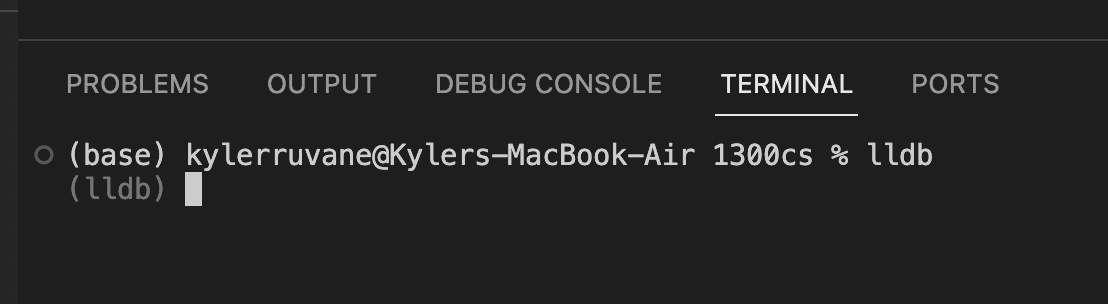
\includegraphics[width=\textwidth]{images/macDebuggerSetup/debugger_mac_1.png}

You can exit this program by typing

\begin{minted}{bash}
    exit
\end{minted}

If it is not installed, your mac should prompt you if you want to install it. Say yes and go through the install. Verify it is installed by typing lldb in your terminal again and seeing the above screenshot.

\subsubsection{Step 3: Install VSCode Extension: CodeLLDB}

Open the extensions tab on the left of VS Code and Search ``CodeLLDB" and click install for the top result shown below.

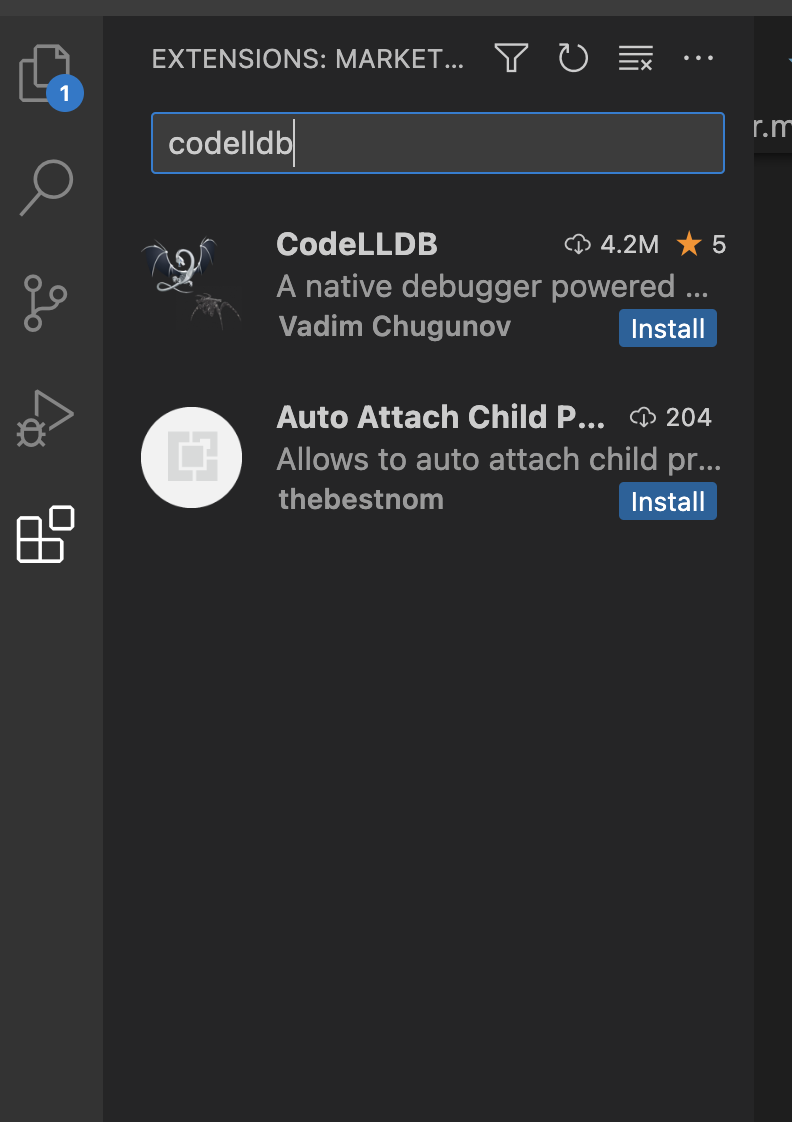
\includegraphics[width=0.3\textwidth]{images/macDebuggerSetup/debugger_mac_2.png}

\subsubsection{Step 4: Click the ``Run and Debug" Tab}

If this is the first time you are using this tab, it will look like this:

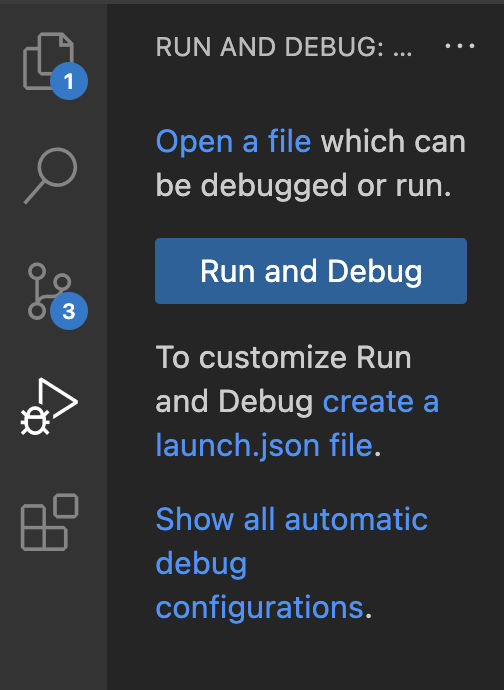
\includegraphics[width=0.3\textwidth]{images/macDebuggerSetup/debugger_mac_3.png}

Press ``create a launch.json file", and then choose the second option ``LLDB".

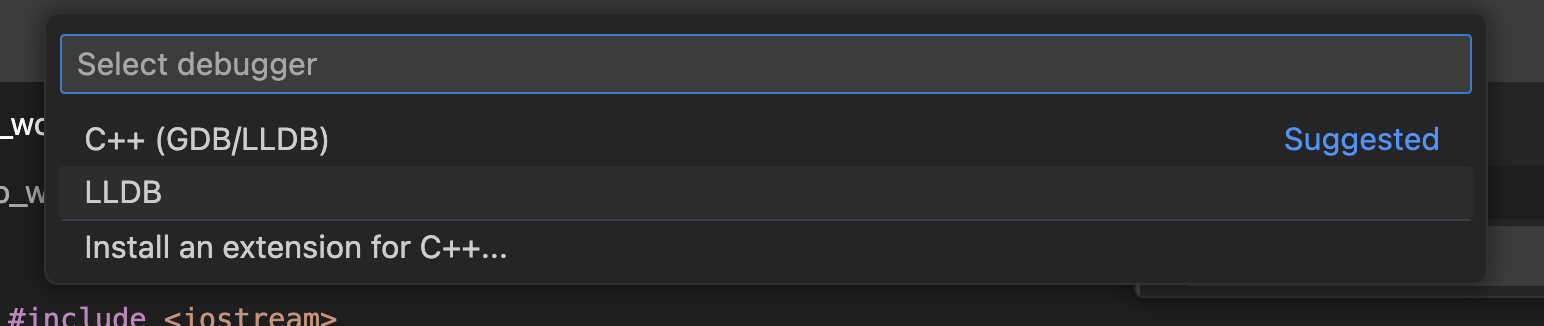
\includegraphics[width=\textwidth]{images/macDebuggerSetup/debugger_mac_4.png}

This should open a new file called ``launch.json".

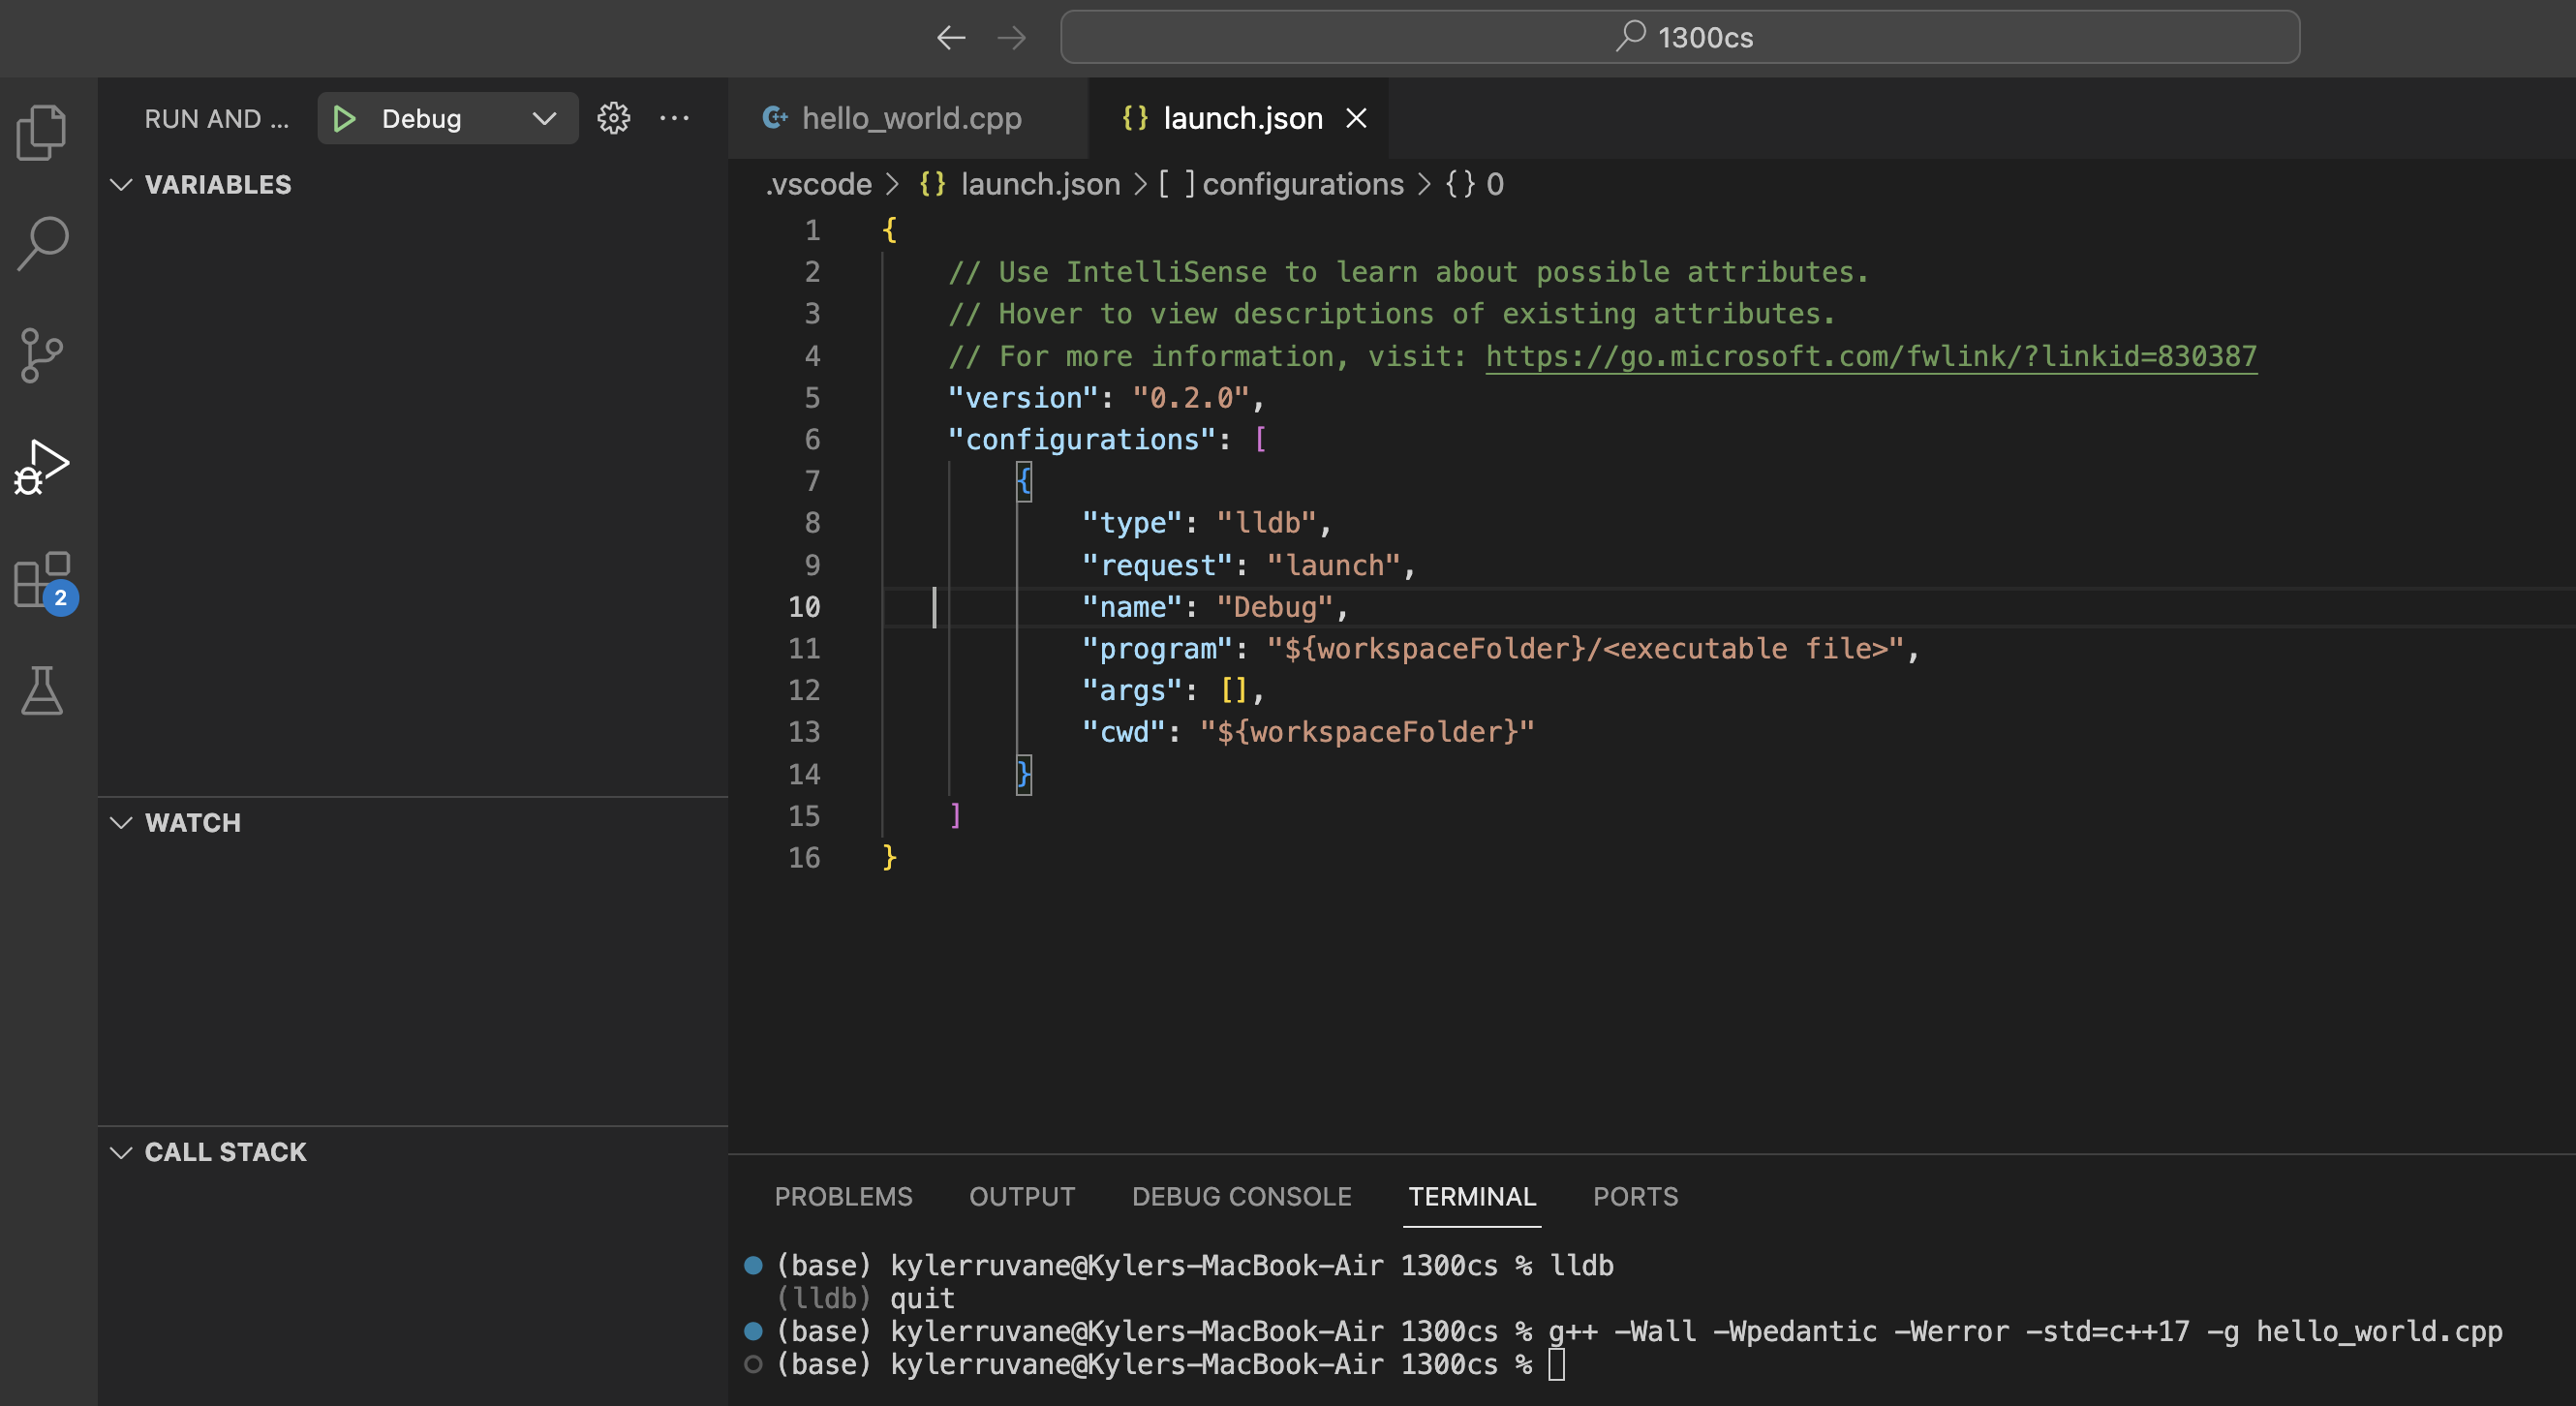
\includegraphics[width=\textwidth]{images/macDebuggerSetup/debugger_mac_5.png}

Delete everything in this file and replace it with:

\begin{minted}{bash}
{
    "version": "0.2.0",
    "configurations": [
        {
            "type": "lldb",
            "request": "launch",
            "name": "a.out debug",
            "program": "${workspaceFolder}/a.out",
            "args": [ ],
            "cwd": "${workspaceFolder}"
        }
    ]
}
\end{minted}

Save the file with "Command + S" or "File > Save".

\subsubsection{Step 5: Add Breakpoints to your Code}

The red dot to the left of line 6 is a 'breakpoint'. Add your own by hovering your mouse just to the left of the line number you want to add a breakpoint to.

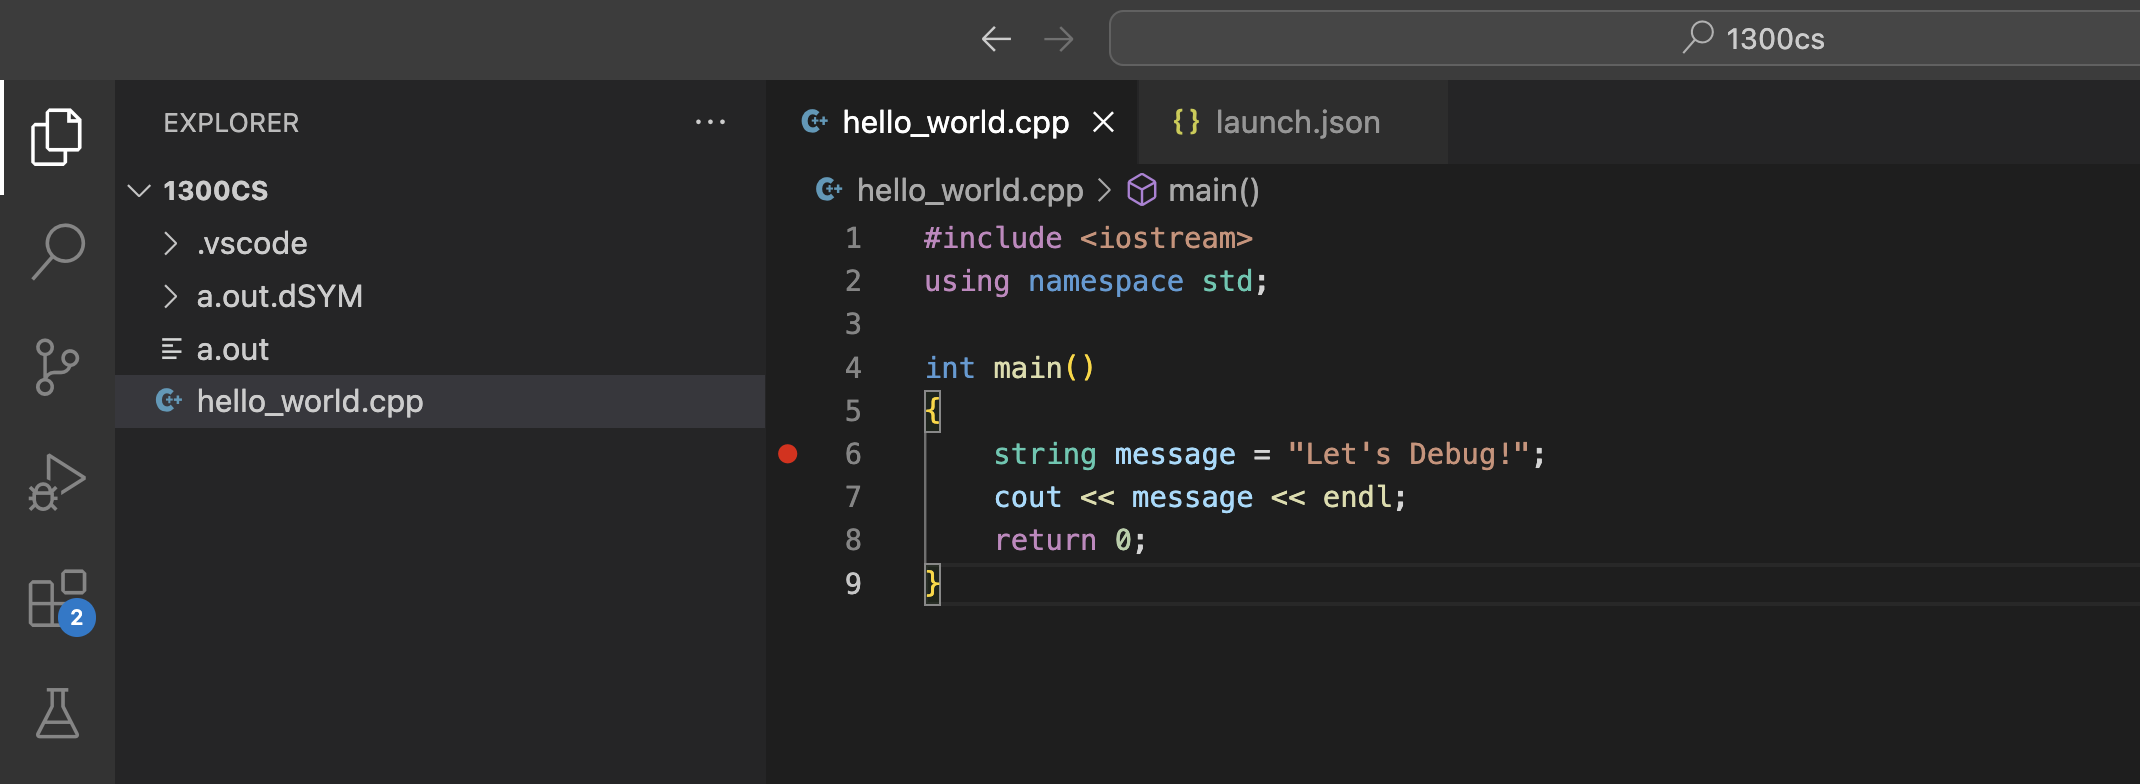
\includegraphics[width=\textwidth]{images/macDebuggerSetup/debugger_mac_6.png}

\subsubsection{Step 6: Compile Your Code with -g}

In your terminal type

\begin{minted}{bash}
    g++ -Wall -Wpedantic -Werror -std=c++17 -g hello_world.cpp
\end{minted}

Note we have added the flag \mintinline{bash}{-g} which tells the compiler to do extra stuff so we can debug the program. You should now see an ``a.out" file and an `a.out.dSYM" folder.

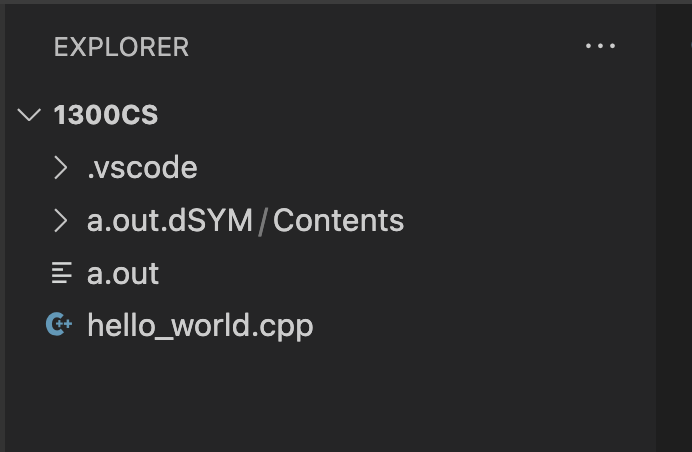
\includegraphics[width=0.3\textwidth]{images/macDebuggerSetup/debugger_mac_7.png}

\subsubsection{Step 7: Press the ``Run and Debug" tab}

This is the sideways triangle with a lady-bug on it.

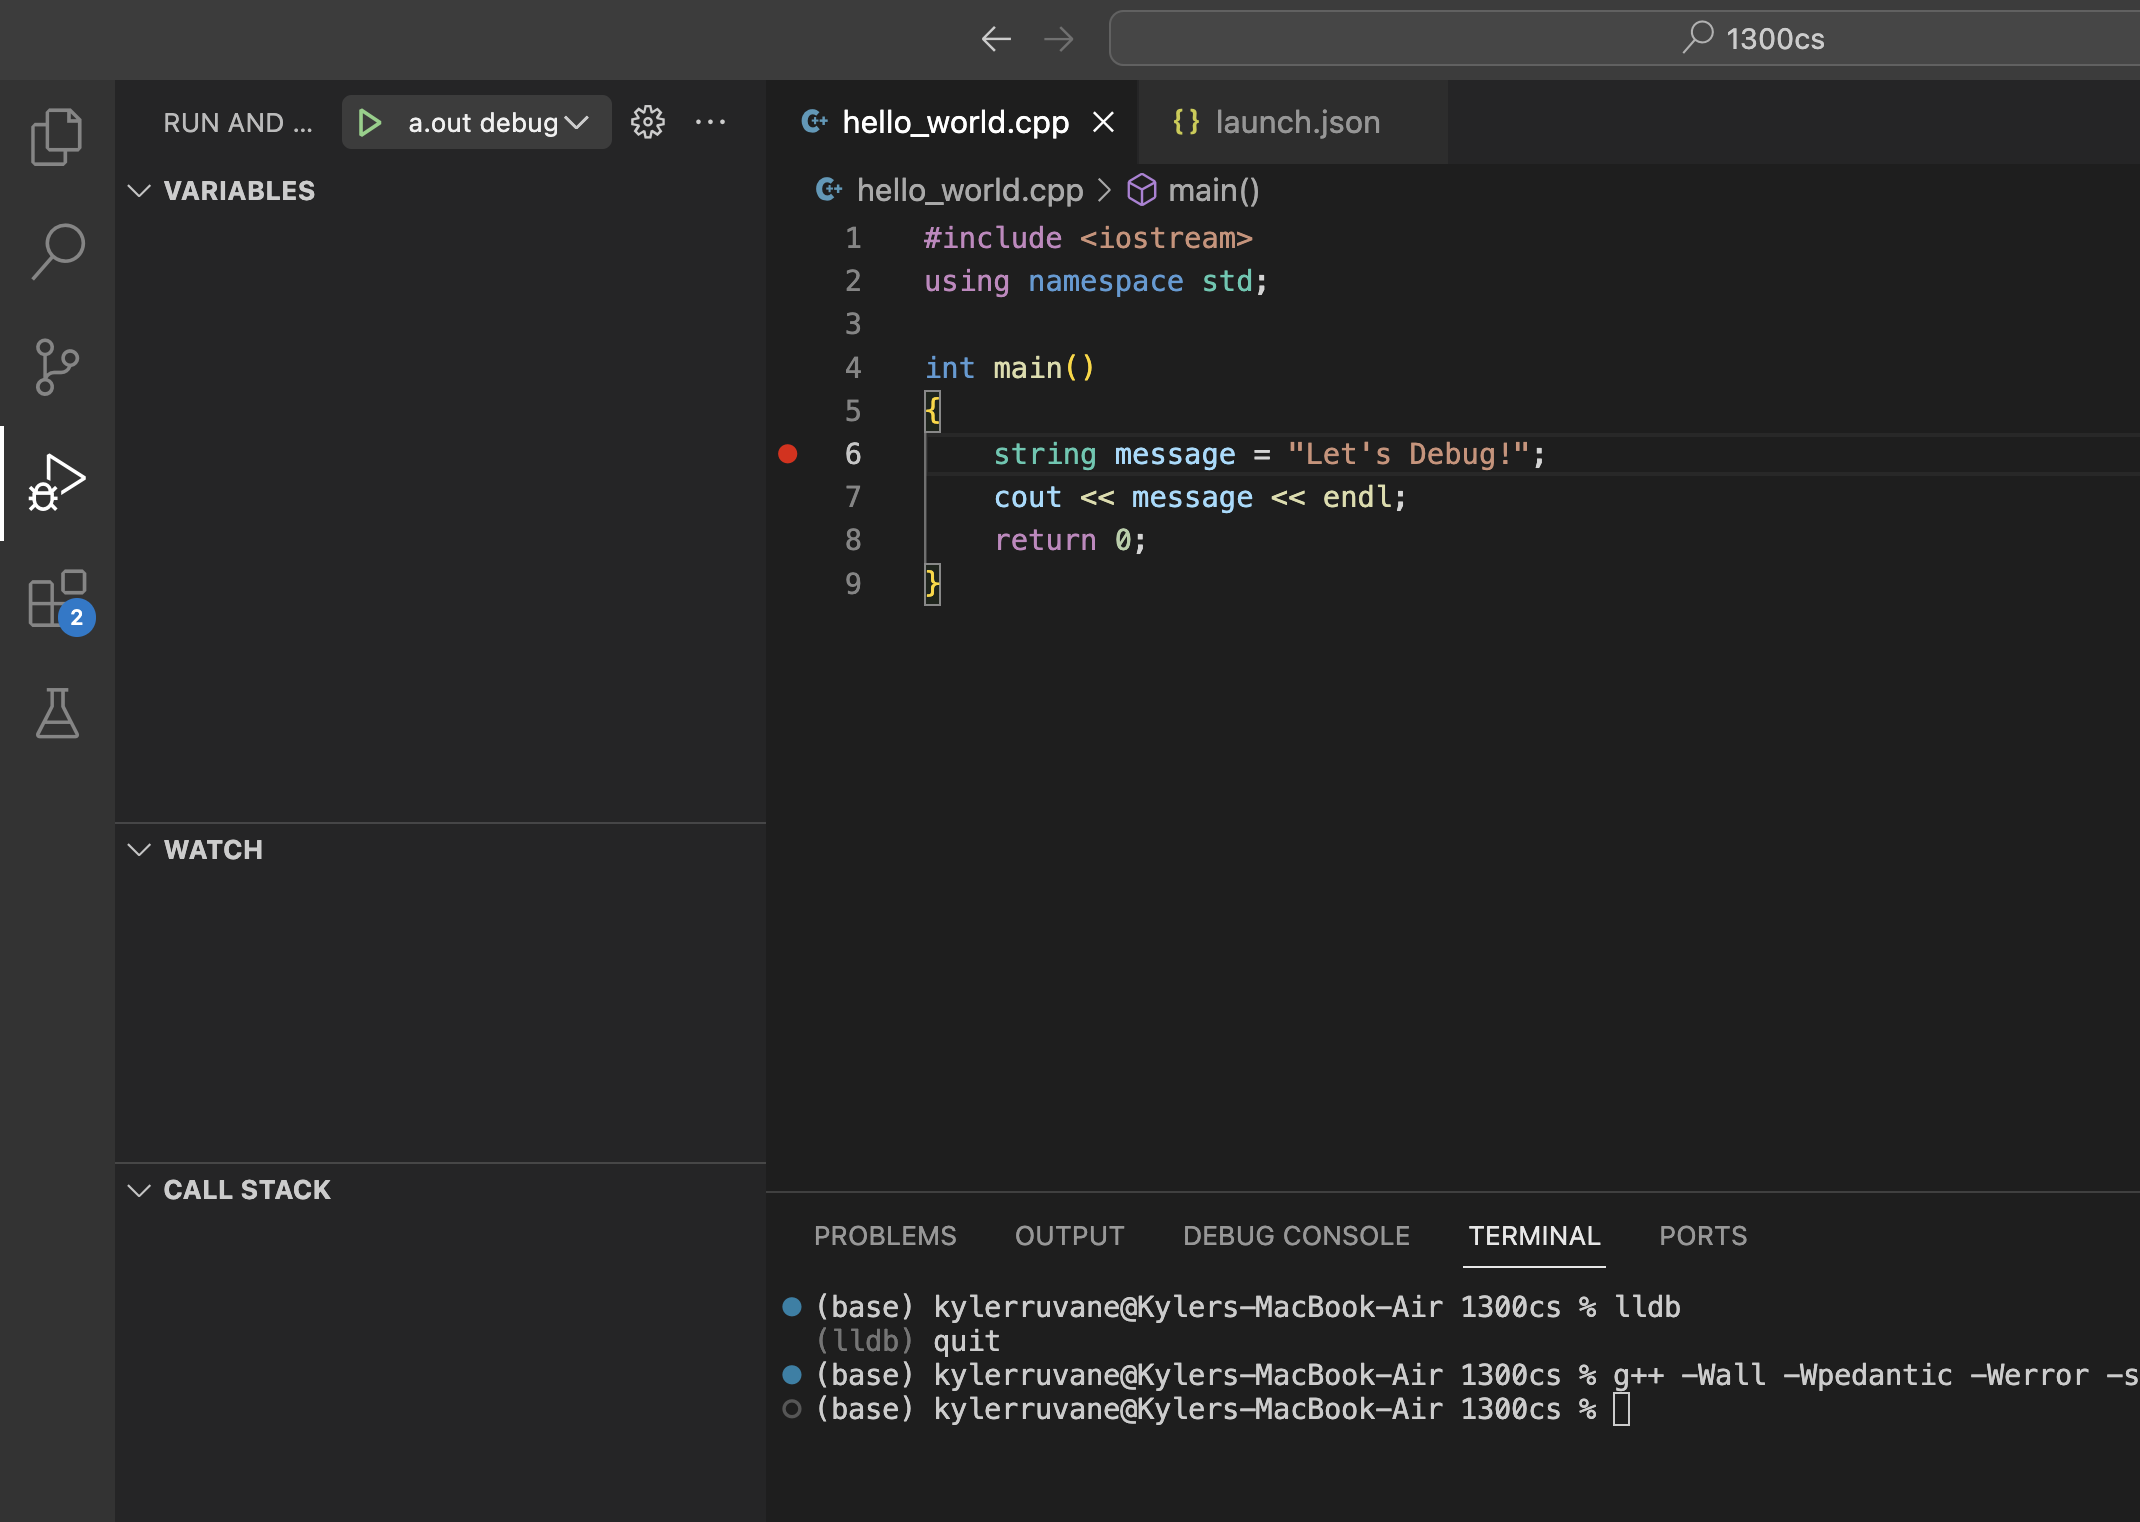
\includegraphics[width=\textwidth]{images/macDebuggerSetup/debugger_mac_8.png}

\subsubsection{Step 8: Press the ``a.out" Green Triangle Button}

You are now debugging!

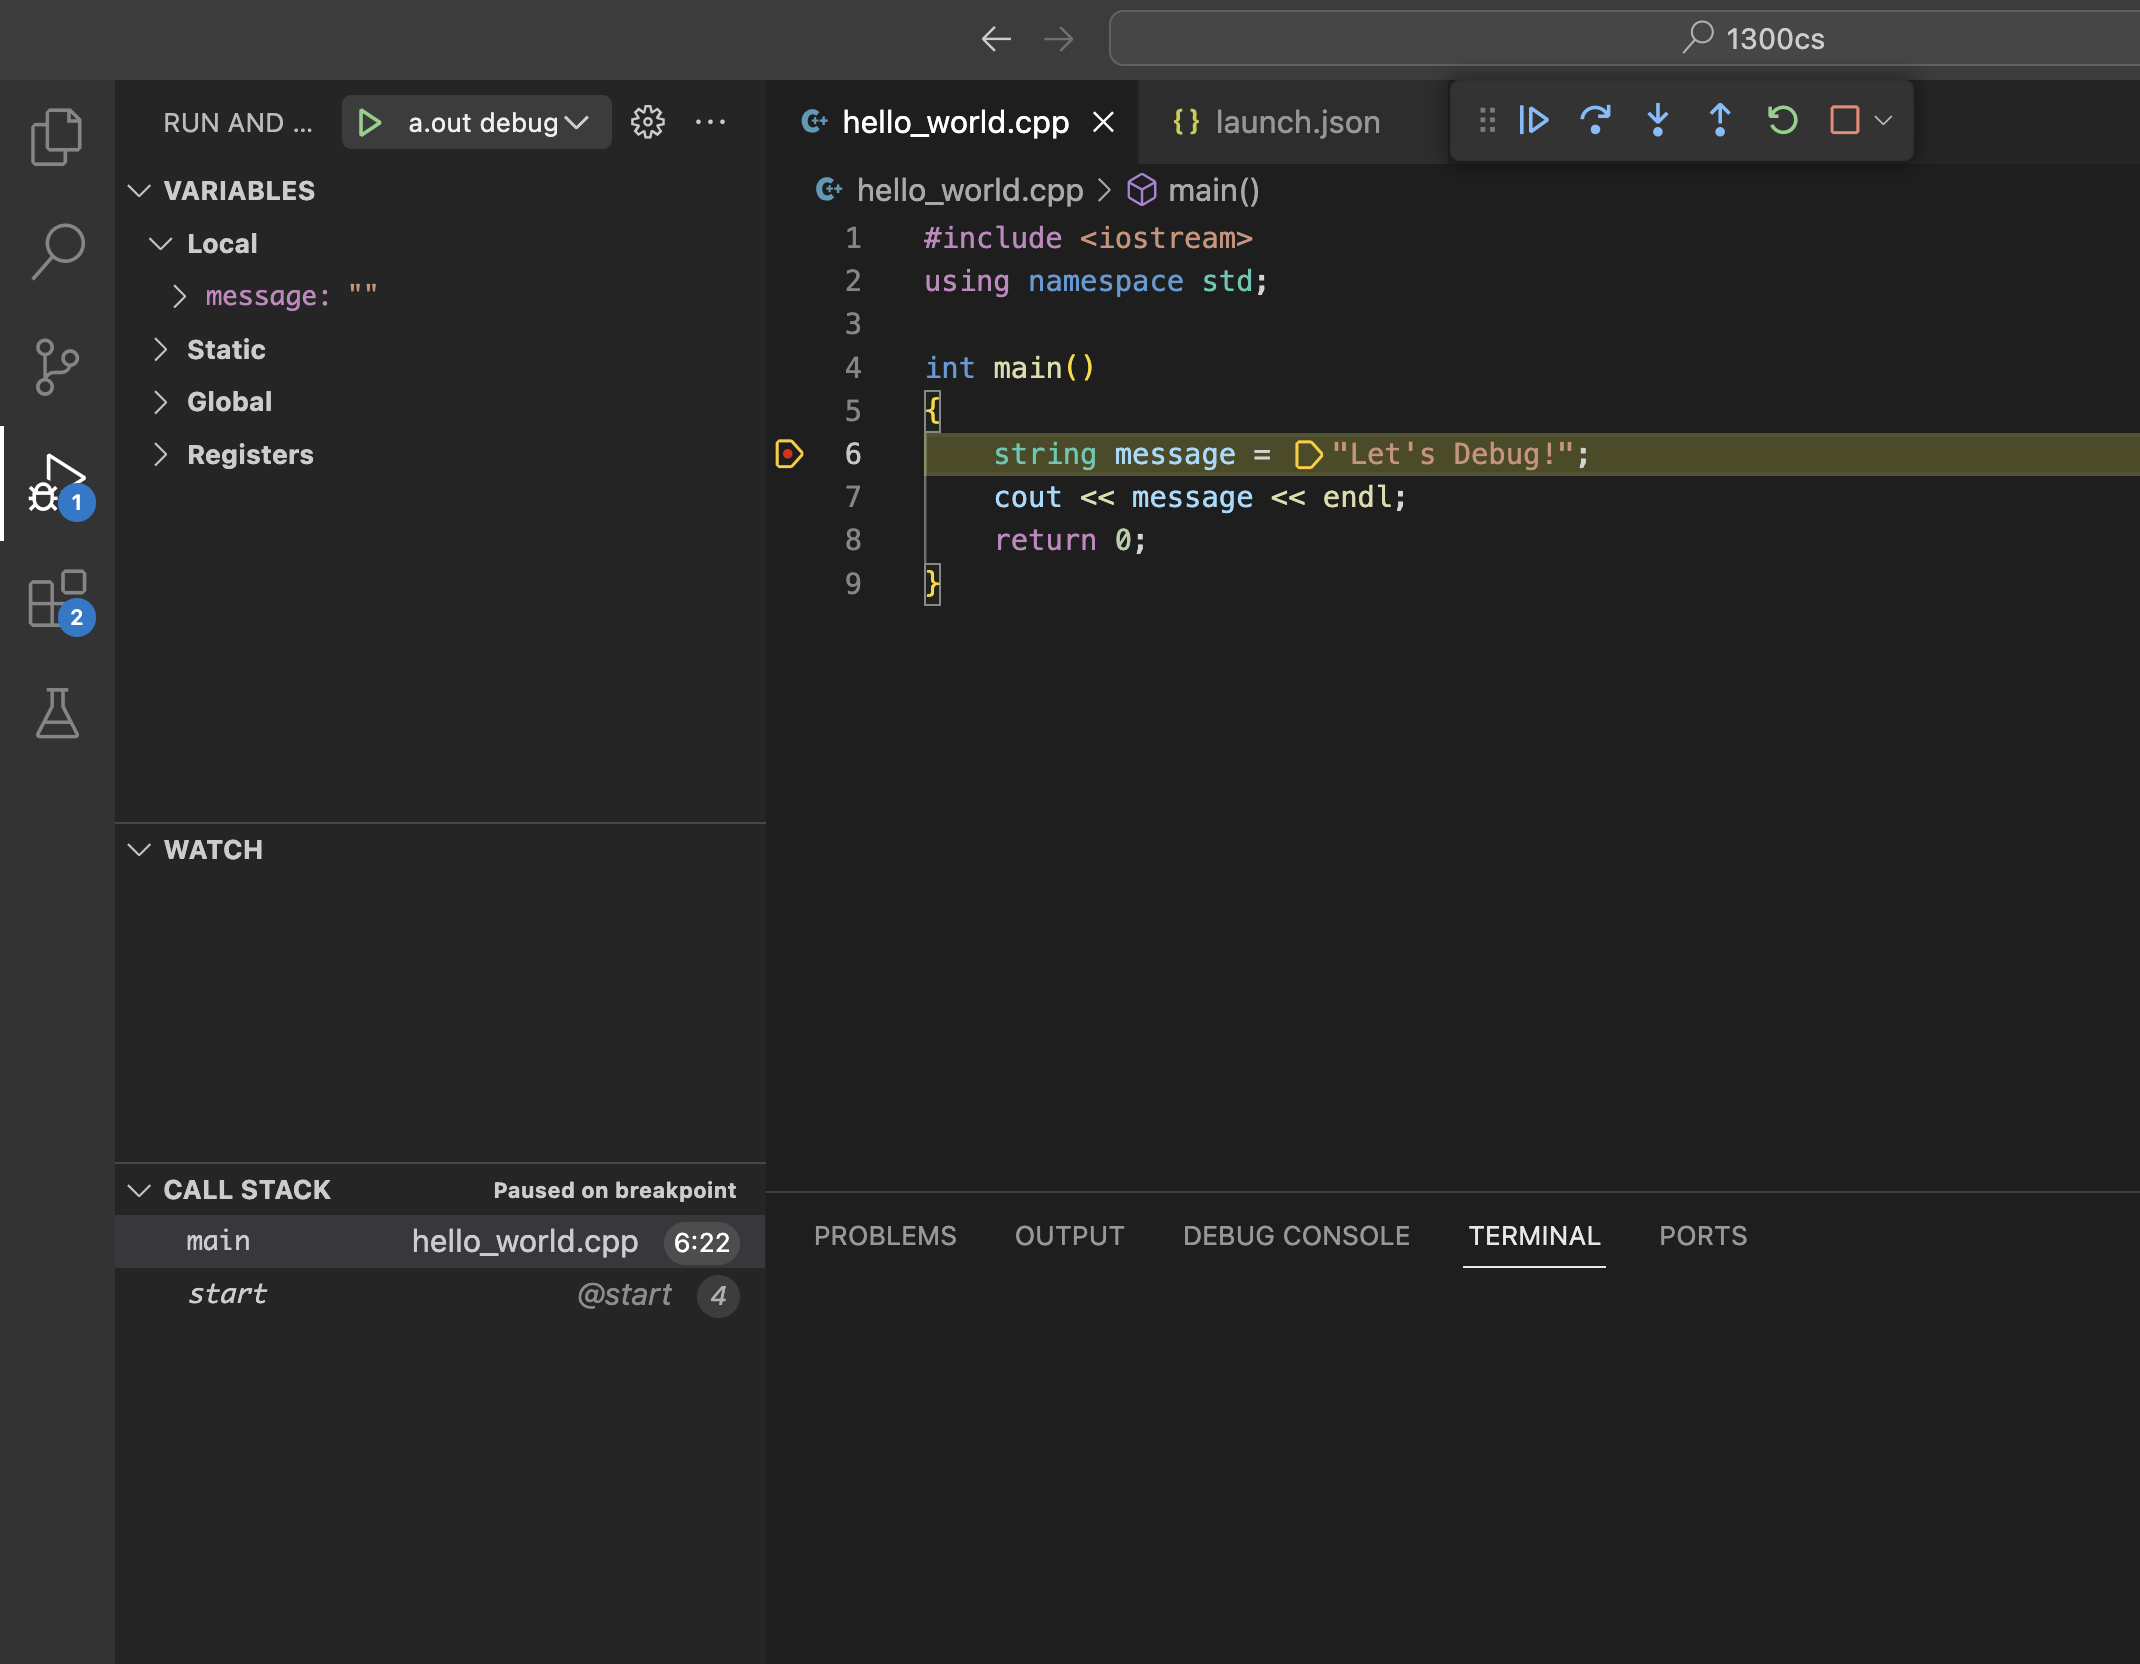
\includegraphics[width=\textwidth]{images/macDebuggerSetup/debugger_mac_9.png}

\subsubsection{Step 9: Control Your Program Live}

Your program will have paused at the first breakpoint it encountered, highlighting the line it is stuck on. Use the control panel to slowly walk through your code execution. The control panel looks like this:

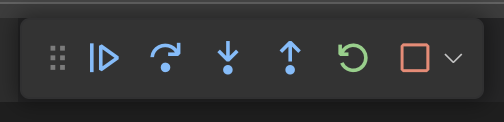
\includegraphics[width=0.3\textwidth]{images/macDebuggerSetup/debugger_mac_10.png}

The buttons, left to right, are:

\begin{itemize}
    \item Continue: go until the next breakpoint is encountered
    \item Step Over: go to the next line, skipping the details of functions
    \item Step Into: go to the next line, if necessary jumping into a function that is called
    \item Step Out: jump to the end of the function your are in, returning to wherever that function was called from
    \item Restart: start the program over from the beginning
    \item Stop: quit debugging
\end{itemize}

Most of the time you can do most of your debugging with just the Continue and the Step Over buttons as long as you have put breakpoints at all the points of your code you care about.

\subsubsection{What Should I Look For?}

The most important two pieces of information you get from debugging is 1. What lines of code are being executed when I run it and 2. What are the values of my variables during execution.

For 1. you can see this in the main .cpp file with the active line being highlighted yellow.

For 2. you can see this in the left panel where all of your in-scope variables will be listed with their value. You can see how their value changes as you step through the program execution.

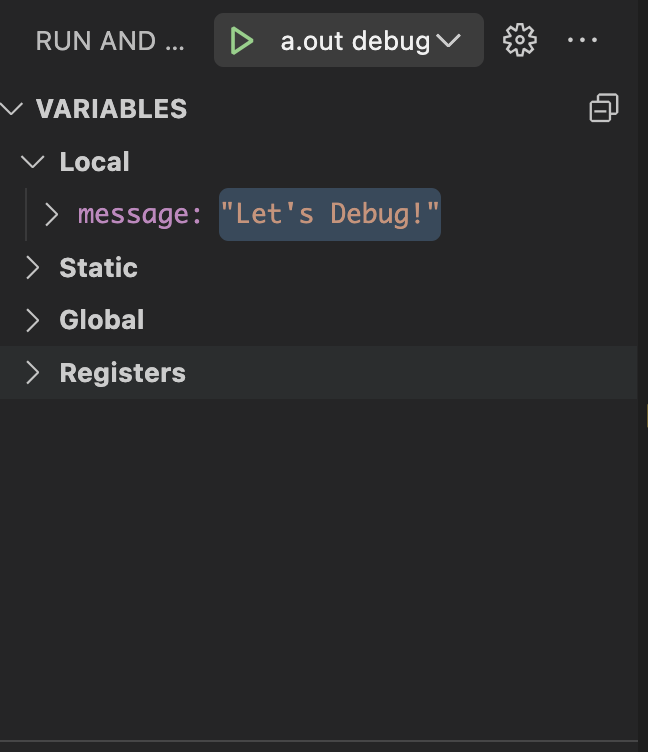
\includegraphics[width=0.3\textwidth]{images/macDebuggerSetup/debugger_mac_11.png}